% Options for packages loaded elsewhere
\PassOptionsToPackage{unicode}{hyperref}
\PassOptionsToPackage{hyphens}{url}
%
\documentclass[
]{article}
\usepackage{amsmath,amssymb}
\usepackage{iftex}
\ifPDFTeX
  \usepackage[T1]{fontenc}
  \usepackage[utf8]{inputenc}
  \usepackage{textcomp} % provide euro and other symbols
\else % if luatex or xetex
  \usepackage{unicode-math} % this also loads fontspec
  \defaultfontfeatures{Scale=MatchLowercase}
  \defaultfontfeatures[\rmfamily]{Ligatures=TeX,Scale=1}
\fi
\usepackage{lmodern}
\ifPDFTeX\else
  % xetex/luatex font selection
\fi
% Use upquote if available, for straight quotes in verbatim environments
\IfFileExists{upquote.sty}{\usepackage{upquote}}{}
\IfFileExists{microtype.sty}{% use microtype if available
  \usepackage[]{microtype}
  \UseMicrotypeSet[protrusion]{basicmath} % disable protrusion for tt fonts
}{}
\makeatletter
\@ifundefined{KOMAClassName}{% if non-KOMA class
  \IfFileExists{parskip.sty}{%
    \usepackage{parskip}
  }{% else
    \setlength{\parindent}{0pt}
    \setlength{\parskip}{6pt plus 2pt minus 1pt}}
}{% if KOMA class
  \KOMAoptions{parskip=half}}
\makeatother
\usepackage{xcolor}
\usepackage[margin=1in]{geometry}
\usepackage{longtable,booktabs,array}
\usepackage{calc} % for calculating minipage widths
% Correct order of tables after \paragraph or \subparagraph
\usepackage{etoolbox}
\makeatletter
\patchcmd\longtable{\par}{\if@noskipsec\mbox{}\fi\par}{}{}
\makeatother
% Allow footnotes in longtable head/foot
\IfFileExists{footnotehyper.sty}{\usepackage{footnotehyper}}{\usepackage{footnote}}
\makesavenoteenv{longtable}
\usepackage{graphicx}
\makeatletter
\def\maxwidth{\ifdim\Gin@nat@width>\linewidth\linewidth\else\Gin@nat@width\fi}
\def\maxheight{\ifdim\Gin@nat@height>\textheight\textheight\else\Gin@nat@height\fi}
\makeatother
% Scale images if necessary, so that they will not overflow the page
% margins by default, and it is still possible to overwrite the defaults
% using explicit options in \includegraphics[width, height, ...]{}
\setkeys{Gin}{width=\maxwidth,height=\maxheight,keepaspectratio}
% Set default figure placement to htbp
\makeatletter
\def\fps@figure{htbp}
\makeatother
\setlength{\emergencystretch}{3em} % prevent overfull lines
\providecommand{\tightlist}{%
  \setlength{\itemsep}{0pt}\setlength{\parskip}{0pt}}
\setcounter{secnumdepth}{5}
\usepackage{setspace}
\renewcommand{\baselinestretch}{1.5}
\usepackage{threeparttable}
\usepackage{booktabs}
\usepackage{siunitx}

  \newcolumntype{d}{S[
    input-open-uncertainty=,
    input-close-uncertainty=,
    parse-numbers = false,
    table-align-text-pre=false,
    table-align-text-post=false
  ]}
  
\ifLuaTeX
  \usepackage{selnolig}  % disable illegal ligatures
\fi
\usepackage[]{natbib}
\bibliographystyle{agsm}
\IfFileExists{bookmark.sty}{\usepackage{bookmark}}{\usepackage{hyperref}}
\IfFileExists{xurl.sty}{\usepackage{xurl}}{} % add URL line breaks if available
\urlstyle{same}
\hypersetup{
  pdftitle={Only You: A Field Experiment of Text Message to Prevent Free-riding in Japan Marrow Donor Program},
  pdfauthor={Hiroki Kato; Fumio Ohtake; Saiko Kurosawa; Kazuhiro Yoshiuchi; Takahiro Fukuda},
  hidelinks,
  pdfcreator={LaTeX via pandoc}}

\title{Only You:
A Field Experiment of Text Message to Prevent Free-riding in Japan Marrow Donor Program}
\author{Hiroki Kato\footnote{Hitostubashi Institute for Advanced Study, Hitotsubashi University, Tokyo, Japan.} \and Fumio Ohtake\footnote{Center for Infectious Disease Education and Research (CiDER), Osaka University, Osaka, Japan.} \and Saiko Kurosawa\footnote{Department of Oncology, Ina Central Hospital, Nagano, Japan.} \and Kazuhiro Yoshiuchi\footnote{Graduate School of Medicine, Tokyo University, Tokyo, Japan.} \and Takahiro Fukuda\footnote{Department of Hematopoietic Stem Cell Transplantation, National Cancer Center Hospital, Tokyo, Japan.}}
\date{Last updated on October 27, 2023}

\begin{document}
\maketitle
\begin{abstract}
Allogeneic hematopoietic stem cell transplants through the Japan Marrow Donor Program take a long time to become available, and only about half of registered patients receive a transplant. This is because much of the transplant coordination is interrupted before the transplant takes place due to the reluctance of registered donors to donate. In collaboration with the Japan Marrow Donor Program, we conduct a field experiment to test an information provision intervention to increase registered donors' willingness to donate. We estimate the effect of information provision using coordination data for 11,049 matched donors. We find that information about the low number of potential donor matches per patient increases willingness to donate by 25\% among men in their 20s. We also find that information that early coordination increases a patient's transplant rate encourages early responses from women in their 20s. These results suggest that providing information affects only certain genders and ages, and in particular encourages behavioral change among younger donors with better transplant outcomes.
\end{abstract}

\hypertarget{intro}{%
\section{Introduction}\label{intro}}

Allogeneic hematopoietic stem cell transplantation is one of the treatments with the lowest relapse rate for leukemia and other blood diseases. In this treatment, (1) anti-cancer drugs and radiation simultaneously kill tumor cells and healthy hematopoietic stem cells, and (2) healthy hematopoietic stem cells donated by others are transplanted. Transplantation requires that the donor's white blood cell type, called HLA, match the patient's HLA.\footnote{In recent years, transplantation between close relatives with semi-matched HLA, known as haploidentical stem cell transplantation, has become more common. In addition, transplantation of blood cells from the umbilical cord or placenta that connects mother and child (cord blood transplantation) has also increased. Unlike bone marrow transplantation, cord blood transplantation can be performed even if the HLA is not a perfect match. In Japan, bone marrow (or peripheral blood) transplants between unrelated individuals, the focus of this study, will account for 20\% of all transplants performed in FY2021 \citep{JapaneseDataCenterf2022}.} While the probability of a match between two randomly selected individuals is less than 1\%, the probability of a match between siblings is the highest at approximately 30\%. The probability of a match between parents and children is also quite low. If there is no match among relatives, patients must seek a donor outside the immediate family. In Japan, patients usually seek a non-relative donor through the Japan Marrow Donor Program (JMDP). However, coordination through the JMDP takes a long time, and only 60\% of registered patients receive a transplant \citep{Hirakawa2018}. Therefore, it is important to shorten the time to transplantation and increase the transplantation rate of registered patients.

There are two types of donor pool policies that increase transplantation rates. The first are policies that increase the number of potential donors to increase the probability of a match. Compared to patients matched with fewer than four donors, the transplantation rate increases from 45\% to 74\% for patients matched with more than 200 donors \citep{Hirakawa2018}. However, according to \citet{Takanashi2016}, the number of potential donors nearly doubled from 2000 to 2015, but the probability of a first-time match increased by only about 5\%.\footnote{This is because the probability of a new donor with a rare HLA type is low.} The marginal benefit of increasing the number of potential donors is small.

The second intervention increases the proportion of potential donors willing to donate and improves the quality of the donor pool. \citet{Hirakawa2018} found that many coordinations (73\% of those conducted in 2004-2013) were interrupted before the first process of coordination, confirmatory typing, for donor-related reasons (including poor health). In particular, younger donors are less likely to interrupt coordination for health reasons and more likely to interrupt coordination for other personal reasons.\footnote{While 15\% of males in their 20s were suspended due to donor health (history, back pain, undergoing treatment, etc.), 41\% were suspended for reasons other than donor health (inability to contact, unavailability, etc.). In addition, 6\% were interrupted due to lack of family consent, a prerequisite for transplantation.} This is an issue not only in the JMDP, but also in marrow donor programs in other countries \citep{Haylock2022}. If donor reasons other than health are correlated with own intentions, then increasing the number of potential donors with strong donor intentions would increase transplantation rates, and the marginal benefit would be greater than the marginal benefit of increasing the number of potential donors.

Therefore, this study examines the effect of providing information that increases the willingness to donate as one of the measures to improve the quality of the donor pool. When a potential donor registered with the JMDP is matched with a specific patient, the matched donor receives a compatibility notice from the JMDP. Matched donors who respond to the notice by indicating their willingness to donate are then coordinated for transplantation. We added two new messages to the compatibility notice based on information published by the JMDP and conducted a field experiment in collaboration with the JMDP to test the effect of the additional messages.

The first message indicates that the number of HLA compatible donors per patient is low. If there are other potential donors with the same HLA type in the pool, one's own donation can be substituted for that compatible donor. In addition, multiple donors (up to 10) can be coordinated for a single patient at the same time. Thus, transplantation through the JMDP is in the nature of a public good. Donors who gain utility from the patient's survival will be more reluctant to donate the more common the HLA. In other words, JMDP-mediated transplantation faces the standard ``free-ride'' problem \citep{Bergstrom2009}.

This problem is essentially the same as the volunteer dilemma, a situation in which public goods are produced by the cooperative behavior of only one person. In the volunteer dilemma, theory predicts that the probability of cooperative behavior by even one person decreases with group size, and this hypothesis has been confirmed in laboratory experiments \citep{Diekmann1985, Diekmann1986, Franzen1999, Davis2017}. In addition, an interview study of previously matched donors \citep{Kurosawa2022} found that those with low donation intentions felt that they were ``one of several donors,'' implying that the fact that their donation could be substituted by others discouraged them from donating. An important difference from the volunteer dilemma is that potential donors in the JMDP cannot know their own HLA type or the number of matched donors at the same time, so they cannot accurately guess the size of the group. As a result, potential donors may overestimate the number of other possible substitutes and be reluctant to donate. The first message aims to correct the behavior resulting from this misperception.

The second message presents the information that early coordination would increase the patient's transplant rate. This message is expected to prevent time-inconsistent donor delaying behavior. Time inconsistency is caused by present bias, one of the key findings of behavioral economics \citep{Laibson1997, ODonoghue2001}. Future utility is over-discounted when comparing the present to the future, rather than the near and distant future, even with the same time lag. Thus, time-inconsistent donors actually delay responding even though they believe in advance that they should respond immediately. The second message shows that the utility of transplantation decreases over time (regardless of the individual's time preference) and aims to change the behavior of the time-inconsistent donor.

We created four experimental arms to test the effects of the above messages. The first experimental arm sent the compatibility notice without the above two messages to matched donors (control group). The second and third experimental arms each added one of the above messages to the compatibility notice. The fourth experimental arm added both messages to the compatibility notice.\footnote{This experimental arm is designed to test the hypothesis that the simultaneous addition of two intervention messages may cause the matched donor to receive excessive information and suffer from cognitive overload.} We conducted a field experiment with 11,154 matched donors who received the compatibility notice between September 2021 and February 2022. We assigned participants to the experimental arms using weekly cluster randomization. We received coordination data at the end of June 2022, in collaboration with JMDP, to test the effects of the messages.

The experiment found that the intervention messages only affected certain genders and age groups. There are two main findings from this study. First, providing only the information that there are fewer HLA-matched donors per patient increases willingness to donate among men in their 20s, but has no statistically significant effect on willingness to donate among other genders or age groups. Second, providing information that the sooner a donor is found, the higher the transplant rate, does not affect the overall response rate for women in their 20s, but does increase responses within 4 days of sending the compatibility notice.\footnote{JMDP recommends a response to the compatibility notice within 7 days.} In other words, this information shortens the number of days to respond rather than encouraging response behavior itself. This effect is not observed for other genders or ages.

This study suggests that information can increase the willingness of potential donors to donate, providing practical insights for marrow donor programs around the world, including the JMDP. Similar to the JMDP, the German-based international marrow donor program, DKMS, and the U.S. marrow donor program, NMDP, have steadily increased their enrollment, but have faced challenges in keeping enrollees motivated and achieving coordination \citep{Switzer1999, Switzer2004, Haylock2022}. Previous studies have examined the effectiveness of donor leave laws \citep{Lacetera2014} and DKMS's own efforts to maintain donor motivation \citep{Haylock2022}.

\citet{Switzer2018} applied an intervention to a message sent by the NMDP when they ask matched potential donors to donate. Their intervention was a message that said, ``Based on the information we currently have, you are in the unique position of likely being a perfect match for this patient,'' which was delivered over the phone to the potential donor whose HLA was a perfect match. Their experiment was not a fully randomized controlled trial and showed that this novel message did not increase the number of coordinations. Although our intervention is very close to this study, we show that the message effect is quite heterogeneous, affecting only certain genders and ages.

In addition, this study contributes to the economic study of costly prosocial behavior such as blood donation. Although stem cell transplantation and blood donation have some similarities, there are also some differences. In the case of blood donation, the time of the intention to donate and the time of the actual donation are the same, whereas in the case of stem cell transplantation, the two time points are different. Therefore, as mentioned earlier, maintaining the willingness of potential donors is a challenge for marrow donor programs. In the context of blood donation, previous studies have examined monetary incentives and non-monetary incentives such as symbolic rewards \citep{Mellstrom2008, Lacetera2010}. As with stem cell transplantation, blood donation can also be considered a public good. \citet{Wildman2009} used data on blood donors only and showed that free riding does not occur. In contrast, our study shows that information about the low number of HLA-compatible donors per patient increases the willingness of men in their 20s to donate, suggesting that they overestimate the number of HLA-compatible donors and engage in free-riding.

This paper is organized as follows. Section \ref{experiment} provides an overview of the coordination process in the JMDP and details the field experiments; Section \ref{result} presents the results; and Section \ref{conclusion} provides discussion and conclusions.

\hypertarget{experiment}{%
\section{Field Experiment}\label{experiment}}

\hypertarget{background}{%
\subsection{Background: Coordination Process of JMDP}\label{background}}

For a better understanding of the timing of our interventions and our data, we outline the coordination process leading up to the donation of stem cells by potential donors enrolled in the JMDP. First, when a potential donor is matched with a patient enrolled in the JMDP, the JMDP office sends the donor the compatibility notice requesting a stem cell donation.\footnote{At the same time, the JMDP office sends a social networking message to the matched donors informing them that JMDP has sent the compatibility notice.} The matched donor fills out a questionnaire and responds to the compatibility notice, indicating his or her willingness to donate.

Coordination for the transplant then begins. The matched donor undergoes confirmatory typing within approximately one month. At this time, the coordinator explains the details of the donation process and asks the matched donors and their families about their willingness to donate. Matched donors can choose between two collection methods (bone marrow or peripheral blood stem cell collection). In addition, the coordinating physician conducts an interview, medical examination and blood draw to test for infection and blood type. These tests are performed to determine if the matched donor meets the criteria established by the JMDP.

Patients can be matched with up to 10 compatible donors at one time. The patient's physician selects the most appropriate candidate from the matched donors who have undergone the confirmatory typing. Importantly, the matched donor does not have access to any information about the matched patient (e.g., how many other matched donors are available). Nor can the matched donor obtain this information from the coordinator or coordinating physician.

The matched donor who is selected as the best donor must give final consent after being informed by the coordinator and coordinating physician. At the same time, a representative of the donor's family must also consent to the donation. After this, the selected donor cannot change his or her mind. After the final consent is given, the selected donor admits him/herself to hospital for approximately one week to undergo pre-operative examinations and preparation for the donation. The donor then undergoes a surgical procedure to collect the stem cells. The time from the confirmatory test to the collection is approximately 3--4 months.

\hypertarget{design}{%
\subsection{Experimental Design}\label{design}}

Our experiment intervenes in the content of the compatibility notice in which JMDP requests a stem cell donation from a matched donor. The standard compatibility notice is as follows.

\begin{quote}
We inform you that your HLA type (white blood cell type) matches that of a patient on our registry and you have been selected as one of our potential donors. We are contacting you to ask if you would like to undergo further testing and interviews in preparation for donation. Please read the enclosed materials carefully, consider whether coordination is possible, and return the form \emph{within 7 days} of receiving this information. {[}Insert intervention messages here{]} If we proceed with the coordination after receiving your return, a coordinator will contact you by phone to discuss the details of your request.
\end{quote}

The standard compatibility notice should be responded to by the donor within 7 days. JMDP also encloses a handbook that describes the coordination process outlined in the previous subsection, as well as the medical questionnaire and donor consent form.

We have added two messages (Probability message and Early Coordination message) to the compatibility notice to facilitate coordination.\footnote{In designing our intervention messages, we have been careful to avoid putting undue psychological pressure on potential donors. Specifically, first, we avoid language that sounds like an appeal. Second, we only use information that is publicly available from the JMDP. In addition, the risks of transplantation are explained in the usual way. The intervention message was approved by the Institutional Review Board of the Graduate School of Economics, Osaka University and the JMDP.} The Probability message is as follows.

\begin{quote}
The number of registered donors whose HLA type matches that of a single registered patient is one in hundreds to tens of thousands. We hope you understand that while we may find more than one potential donor, it is not a large number.
\end{quote}

This message emphasizes the low number of matched donors per registered patient. Transplantation is a public good in the sense that if there are other potential donors with the same HLA type in the pool, one's own donation can be substituted for that compatible donor. Thus, as predicted by the volunteer dilemma, the more common the HLA type, the more reluctant the donor will be to donate.

In the context of stem cell transplantation, however, the expectation of the size of the group influences the decision, because a matched donor cannot know the exact size of the group. Therefore, the higher a donor's expectation of the number of potential donors with the same HLA type, the more reluctant he or she will be to donate. If a donor's beliefs are too high, the Probability message would discourage free-riding and increase willingness to donate by adjusting beliefs downward. The opposite effect is also possible. If the donor's beliefs are underestimated, the Probability message may induce free-riding and reduce donation intentions by adjusting beliefs upward.

The Early Coordination message is as follows.

\begin{quote}
About 60\% of patients are able to receive a transplant through the Japan Marrow Donor Program. The earlier a donor can be found to donate bone marrow, the higher that percentage can be.
\end{quote}

This message is expected to work with time-inconsistent matched donors. Time-inconsistent donors may think it is optimal to respond immediately in advance, but actually delay their response. This message suggests that early coordination increases the rate of transplantation for the patient, and that the utility of transplantation decays over time (regardless of the individual's time preference). Time-inconsistent donors who read this message may recognize that delaying a response does not increase utility and may change their decision to respond immediately. Thus, this message is expected to increase the response rate over a short period of time.

We set up four experimental groups to estimate the effects of the two intervention messages. Experimental arm A received a standard compatibility notice with no intervention messages (control group). Experimental arms B and C received the notice with the Probability message and the Early Coordination message, respectively. Experimental arm D received the notice with two intervention messages added at the same time. This experimental arm was designed to test the negative effects of cognitive load caused by information overload.

\begin{table}

\caption{\label{tab:assignment}Assignment Schedule}
\centering
\fontsize{9}{11}\selectfont
\begin{threeparttable}
\begin{tabular}[t]{lcccccc}
\toprule
week & Sep 21 & Oct 21 & Nov 21 & Dec 21 & Jan 22 & Feb 22\\
\midrule
Week 1 & B & C & C & D & B & A\\
Week 2 & D & B & A & A & C & B\\
Week 3 & A & D & B & C & D & C\\
Week 4 & C & A & D & B & A & D\\
\bottomrule
\end{tabular}
\begin{tablenotes}
\item Notes: See Table \ref{tab:summary} for detail intervention of each experimental arm. Control group is experimental arm A.
\end{tablenotes}
\end{threeparttable}
\end{table}

Participants in the experiment were 11,154 matched donors who received the compatibility notice between September 2021 and February 2022. To maintain randomness to the best of the JMDP office's ability, we assigned experimental groups by cluster randomization on a weekly basis. We designed the experimental groups to be balanced across weeks and months as much as possible. Table \ref{tab:assignment} summarizes the assignment schedule. In conducting the experiment, we obtained approval from the Graduate School of Economics, Osaka University, and the JMDP.

\hypertarget{data-and-empirical-strategy}{%
\subsection{Data and Empirical Strategy}\label{data-and-empirical-strategy}}

JMDP provided the coordination data at the end of June 2022. The unit of observation is the experimental participant. As individual characteristics, the data record gender, age, number of coordination experiences, and prefecture-level residence area. As the coordination process, the data record whether each stage (response to compatibility notice, confirmatory typing, candidate selection, final consent, and collection) was reached. We use these variables as outcome variables. In addition, for responses to the notice, the data record the number of days to respond and the willingness to donate. If coordination was interrupted, the data record the reason for the interruption in three categories (patient reasons, donor non-health reasons, and donor health reasons). The analysis uses 11,049 matched donors living in Japan whose coordination (including interruptions) was completed.\footnote{One matched donor lived abroad. There were 104 matched donors with ongoing coordination at the time of data provision. The proportion of matched donors with ongoing matching is balanced across the experimental arms (F-test, p-value = \(0.383\)).}

As additional data, we use the list of medical institutions published on the Internet by the JMDP.\footnote{\url{https://www.jmdp.or.jp/hospitals/view2/} (access date: August 4, 2022)} This list includes complete addresses, availability of bone marrow collection (BM collection), and availability of peripheral blood stem cell collection (PBSC collection). We aggregated this list at the prefecture level, calculated the number of hospitals per 10 square kilometers, and merged it with the coordination data using the prefecture as the merge key. We consider this variable as the travel cost of coordination and donation.

\begin{table}

\caption{\label{tab:summary}Summary of Field Experiment}
\centering
\fontsize{9}{11}\selectfont
\begin{threeparttable}
\begin{tabular}[t]{lccccc}
\toprule
\multicolumn{1}{c}{ } & \multicolumn{4}{c}{Experimental Arms} & \multicolumn{1}{c}{ } \\
\cmidrule(l{3pt}r{3pt}){2-5}
 & A & B & C & D & F-test, p-value\\
\midrule
\addlinespace[0.3em]
\multicolumn{6}{l}{\textbf{A. Interventions}}\\
\hspace{1em}Standard notification & X & X & X & X & \\
\hspace{1em}Probability message &  & X &  & X & \\
\hspace{1em}Early Coordination message &  &  & X & X & \\
\addlinespace[0.3em]
\multicolumn{6}{l}{\textbf{B. Sample Size}}\\
\hspace{1em}N & 2535 & 3053 & 2726 & 2735 & \\
\addlinespace[0.3em]
\multicolumn{6}{l}{\textbf{C. Balance Test}}\\
\hspace{1em}Male (= 1) & 0.624 & 0.633 & 0.631 & 0.609 & 0.231\\
\hspace{1em}Age & 38.376 & 38.121 & 37.448 & 37.978 & 0.004\\
\hspace{1em}Number of past coordinations & 1.609 & 1.589 & 1.625 & 1.563 & 0.130\\
\hspace{1em}Number of listed hospitals & 0.476 & 0.490 & 0.487 & 0.485 & 0.835\\
\hspace{1em}Number of hospitals listed with PBSC collection & 0.162 & 0.167 & 0.166 & 0.164 & 0.838\\
\hspace{1em}Number of hospitals listed with BM collection & 0.246 & 0.256 & 0.254 & 0.251 & 0.741\\
\bottomrule
\end{tabular}
\begin{tablenotes}
\item Notes: For balance test, we regress a covariate on treatment dummies and test a null hypothesis that all coefficients are zero. We use the robust standard errors for statistical inference.
\end{tablenotes}
\end{threeparttable}
\end{table}

Table \ref{tab:summary} provides a summary of the field experiment. Panel A shows the intervention for each experimental arm, and Panel B shows the sample size for each experimental arm. Panel C is a balanced test of whether randomization was successful. The assignment of experimental arms is approximately random, since there is no average difference between experimental arms for any variable except age. However, age may vary across groups. The average age of experimental arm C is about one year younger than that of the control group.

Since we are interested in what information should be given to all potential donors, we want to identify the average treatment effect. Since the assignment of experimental groups should be independent of the potential outcomes (the outcome variable that would be observed if an experimental group is assigned) conditioned on a predetermined variable, we can identify the average treatment effect by the difference in means across experimental groups conditioned on the predetermined variable. Thus, we estimate the following linear probability model for individual \(i\) who received the compatibility notice in week \(w\) of month \(m\):

\[
  Y_{imw} =
  \beta_1 \cdot \text{B}_{mw} + \beta_2 \cdot \text{C}_{mw} + \beta_3 \cdot \text{D}_{mw}
  + X'_i \gamma + \lambda_m + \theta_w + u_{imw},
\]

where \(X_i\) is a vector of individual characteristics. We add month and week dummy variables \(\lambda_m\) and \(\theta_w\) to control for common shocks at a given time period. Our parameters of interest are \((\beta_1, \beta_2, \beta_3)\). When fixed effects are added, there seems to be no cause to generate correlations within clusters (experimental weeks) of unobservable elements \(u_{imw}\). Thus, we use robust standard errors for statistical inference.\footnote{We conducted a regression analysis with cluster standard errors as a robustness check, confirming no change in the main results presented in this paper.}

\hypertarget{result}{%
\section{Experimental Results}\label{result}}

\hypertarget{intention}{%
\subsection{Effects on Reply and Intention}\label{intention}}

First, we estimate the message effect on responses that are most likely to reflect the donor's intention to donate. The outcome variable for responses is a dummy variable taking one if a donor responded to the compatibility notice regardless of the donor's intention to donate. The response rate for the control group (experimental group A) is \(88.35\)\%.

We decompose the message effect on responses into two effects. The first is the effect on responses associated with the intention to donate. The outcome variable is a dummy variable that takes one if a matched donor responded to the compatibility message and indicated a willingness to donate. The second is the effect on responses without intention. The outcome variable is a dummy variable that takes one if a matched donor responded to the compatibility notice and did not indicate an intention to donate.

In estimating these effects, we code the outcome variable for non-responders as zero and include them in the analysis sample. Thus, the sum of the two outcome variables is always equal to a dummy variable for response, so that the sum of the effects on positive and negative intentions is the effect on response. In the control group, the response rate with positive intentions is \(55.33\)\%, while the response rate with negative intentions is \(33.03\)\%. Thus, \(62.63(=55.33/88.35)\)\% of respondents have the intention to donate.

It is possible that coordination is interrupted for patient reasons before a matched donor responds. Since this happens independently of the matched donor's intentions, we exclude from our analysis sample the \(0.5\)--\(0.7\)\% that fall into such a case in each experimental group.

\begin{table}

\caption{\label{tab:reg-stock}Linear Probability Model of Reply and Intention}
\centering
\fontsize{9}{11}\selectfont
\begin{threeparttable}
\begin{tabular}[t]{lcccccc}
\toprule
\multicolumn{3}{c}{ } & \multicolumn{4}{c}{Intention} \\
\cmidrule(l{3pt}r{3pt}){4-7}
\multicolumn{1}{c}{ } & \multicolumn{2}{c}{Reply} & \multicolumn{2}{c}{Positive} & \multicolumn{2}{c}{Negative} \\
\cmidrule(l{3pt}r{3pt}){2-3} \cmidrule(l{3pt}r{3pt}){4-5} \cmidrule(l{3pt}r{3pt}){6-7}
  & (1) & (2) & (3) & (4) & (5) & (6)\\
\midrule
Treatment B & \num{0.0105} & \num{0.0139}** & \num{0.0218} & \num{0.0210}* & \num{-0.0113} & \num{-0.0071}\\
 & (\num{0.0075}) & (\num{0.0059}) & (\num{0.0135}) & (\num{0.0123}) & (\num{0.0094}) & (\num{0.0076})\\
Treatment C & \num{-0.0057} & \num{0.0026} & \num{-0.0053} & \num{-0.0029} & \num{-0.0004} & \num{0.0054}\\
 & (\num{0.0081}) & (\num{0.0047}) & (\num{0.0151}) & (\num{0.0112}) & (\num{0.0150}) & (\num{0.0094})\\
Treatment D & \num{0.0058} & \num{0.0062} & \num{0.0046} & \num{0.0058} & \num{0.0012} & \num{0.0004}\\
 & (\num{0.0074}) & (\num{0.0052}) & (\num{0.0166}) & (\num{0.0101}) & (\num{0.0138}) & (\num{0.0069})\\
\midrule
Control average & 0.8835 & 0.8835 & 0.5533 & 0.5533 & 0.3303 & 0.3303\\
Covariates &  & X &  & X &  & X\\
Num.Obs. & \num{10985} & \num{10985} & \num{10985} & \num{10985} & \num{10985} & \num{10985}\\
\bottomrule
\end{tabular}
\begin{tablenotes}
\item Notes: * p < 0.1, ** p < 0.05, *** p < 0.01. The robust standard errors are in parentheses. Covariates are gender, squared polynomial of age, number of past coordinations, number of hospitals per 10 square kilometers, number of hospitals with PBSC collection per 10 square kilometers, number of hospitals with BM collection per 10 square kilometers, month dummies, and week dummies.
\end{tablenotes}
\end{threeparttable}
\end{table}

Table \ref{tab:reg-stock} presents the estimation results of the linear probability model. The odd columns include only the experimental group dummy as an explanatory variable, corresponding to a simple difference in means. The even columns control for individual attribute, month and week fixed effects in addition to the experimental arm dummies. The estimated results show that all experimental groups, with and without covariates, have no statistically significant effects on responses and intentions. As an alternative method, we estimate a logit model (Table \ref{tab:logit-stock}) and obtain similar results (95\% confidence intervals for odds ratios include 1).

\begin{figure}[t]
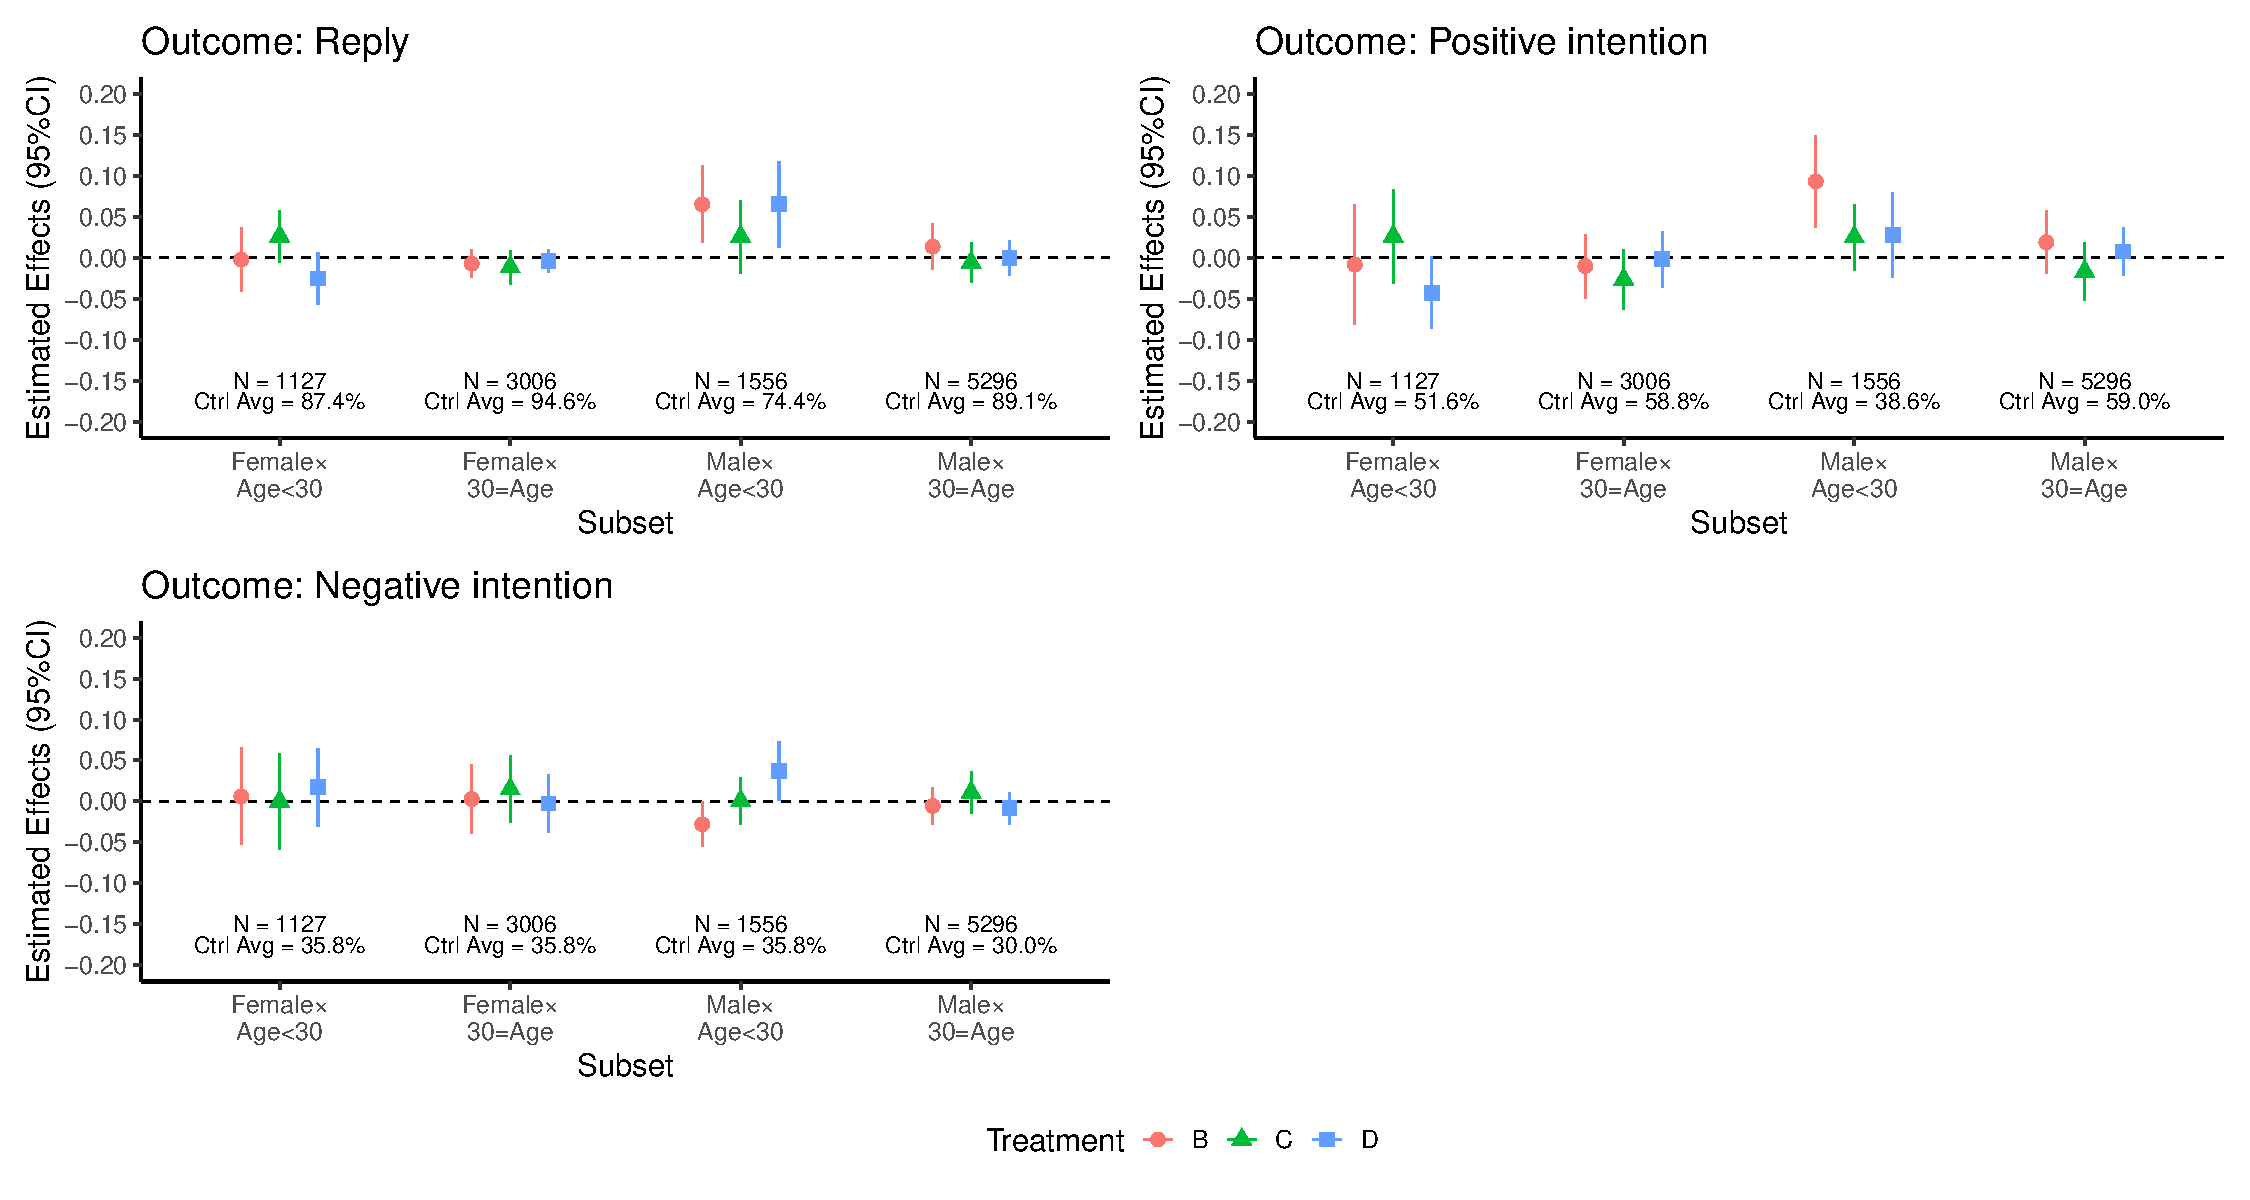
\includegraphics{robustness-body_files/figure-latex/coefplot-reg-stock-subset-1} \caption{Effect on Reply and Intentions by Gender and Age Group. Notes: These plots show the average effect (and associated 95 percent confidential interval) on each outcome by gender and age group. We use robust standard errors We control number of past coordinations, number of hospitals per 10 square kilometers, number of hospitals with PBSC collection per 10 square kilometers, number of hospitals with BM collection per 10 square kilometers, month and week dummies.}\label{fig:coefplot-reg-stock-subset}
\end{figure}

Next, to test for heterogeneity in the message effects, we divide the sample into four subsets by gender and age group (under 30 or not) and estimate the message effects in each subset. Figure \ref{fig:coefplot-reg-stock-subset} shows the coefficient plots. The results show that experimental groups B and D, which include the Probability message, increase the response rate of men in their 20s by about 6 percentage points (\(8.06\)\% increase, since the control mean is \(74.4\)\%), which is statistically significant at the 5\% level. In particular, experimental group B, to which only the Probability message was added, increases responses with positive intentions by about 10 percentage points (\(25.91\)\% increase, since the control mean is \(38.6\)\%), which is also statistically significant. However, for the other gender and age groups, treatment messages have no statistically significant effect on responses and intentions.

In the control group, approximately 50(\(=38.6/74.4\))\% of males in their 20s who responded to the compatibility notice were willing to donate, which is lower than the willingness rate of respondents in the other gender and age groups (60\%).\footnote{For women in their 20s, 59 (\(=51.6/87.4\))\%; for men over 30, 66 (\(=59.0/89.1\))\%; for women over 30, 62 (\(=58.8/94.6\))\%.} Experimental group B (Probability message) raises the intention rate of male respondents in their 20s from 50\% to 60\% (\(=(38.6 + 10)/(74.4 + 6)\)). In addition, young men are reported to have better transplant outcomes than other genders and ages \citep[e.g.,][]{Kollman2016}. Taken together, we can say that the Probability message improves the efficiency of coordination in the sense that it encourages behavioral change (initiation of coordination) in desirable donors.

\hypertarget{rcf}{%
\subsection{Random Causal Forest}\label{rcf}}

To explore the heterogeneity of intervention effects further, we use random causal forests (RCF), which allow us to test the heterogeneity of treatment effects in a fully nonparametric way \citep{Athey2016, Wager2018}. The method is based on a regression tree algorithm and estimates the average treatment effect conditional on observed characteristics. This method has been used in a variety of contexts, including labor \citep{Davis2017}, education \citep{Carlana2022}, and energy conservation \citep{Murakami2022}.

The algorithm splits the sample into two subsamples (leaves) using one of the covariates \(X_j\). Specifically, the algorithm divides the sample into a sample for which \(X_j \le x\) and a sample for which \(X_j > x\). The regression tree determines a specific threshold \(x\) to minimize the mean squared error of the outcome variable. Since the RCF aims to estimate the average treatment effect of a leaf (conditional average treatment effect), the threshold \(x\) is set to minimize the expected mean squared error of the predicted treatment effect. This minimization is achieved by increasing the variance of the conditional mean treatment effect across leaves (heterogeneity) and decreasing the variance within leaves. This splitting process is repeated for each leaf until the termination condition is reached. RCF predicts the conditional mean treatment effect at the terminal leafs.

The disadvantage of the regression tree algorithm is that the variance of the predictions becomes large (overfitting), which reduces the accuracy of the predictions. To prevent this, RCF introduces an algorithm called the ensemble method. It creates thousands of subsamples and grows a tree with each subsample. The final result is the average of the predictions from thousands of trees.\footnote{For technical details, see \citet{Athey2016} and \citet{Wager2018}. This study also uses a technique called generalized random forests, which treats RCF as a special case, but the intuition remains the same. See \citet{Athey2019} and \citet{Athey2019a} for details on generalized random forests.}

Roughly speaking, RCF predicts treatment effect from observed characteristics. In other words, it can predict treatment effects based on individual characteristics, even for individuals who did not receive the intervention. This method must assume that treatment assignment is conditionally independent of the potential outcome variable. Since the experimental group is approximately randomly assigned, we can use this method. In this subsection, we focus on the effect on responses with intentions. The covariates used in the RCF are gender, age, past coordination experience, and the density of hospitals in the area of residence.

\begin{figure}[t]
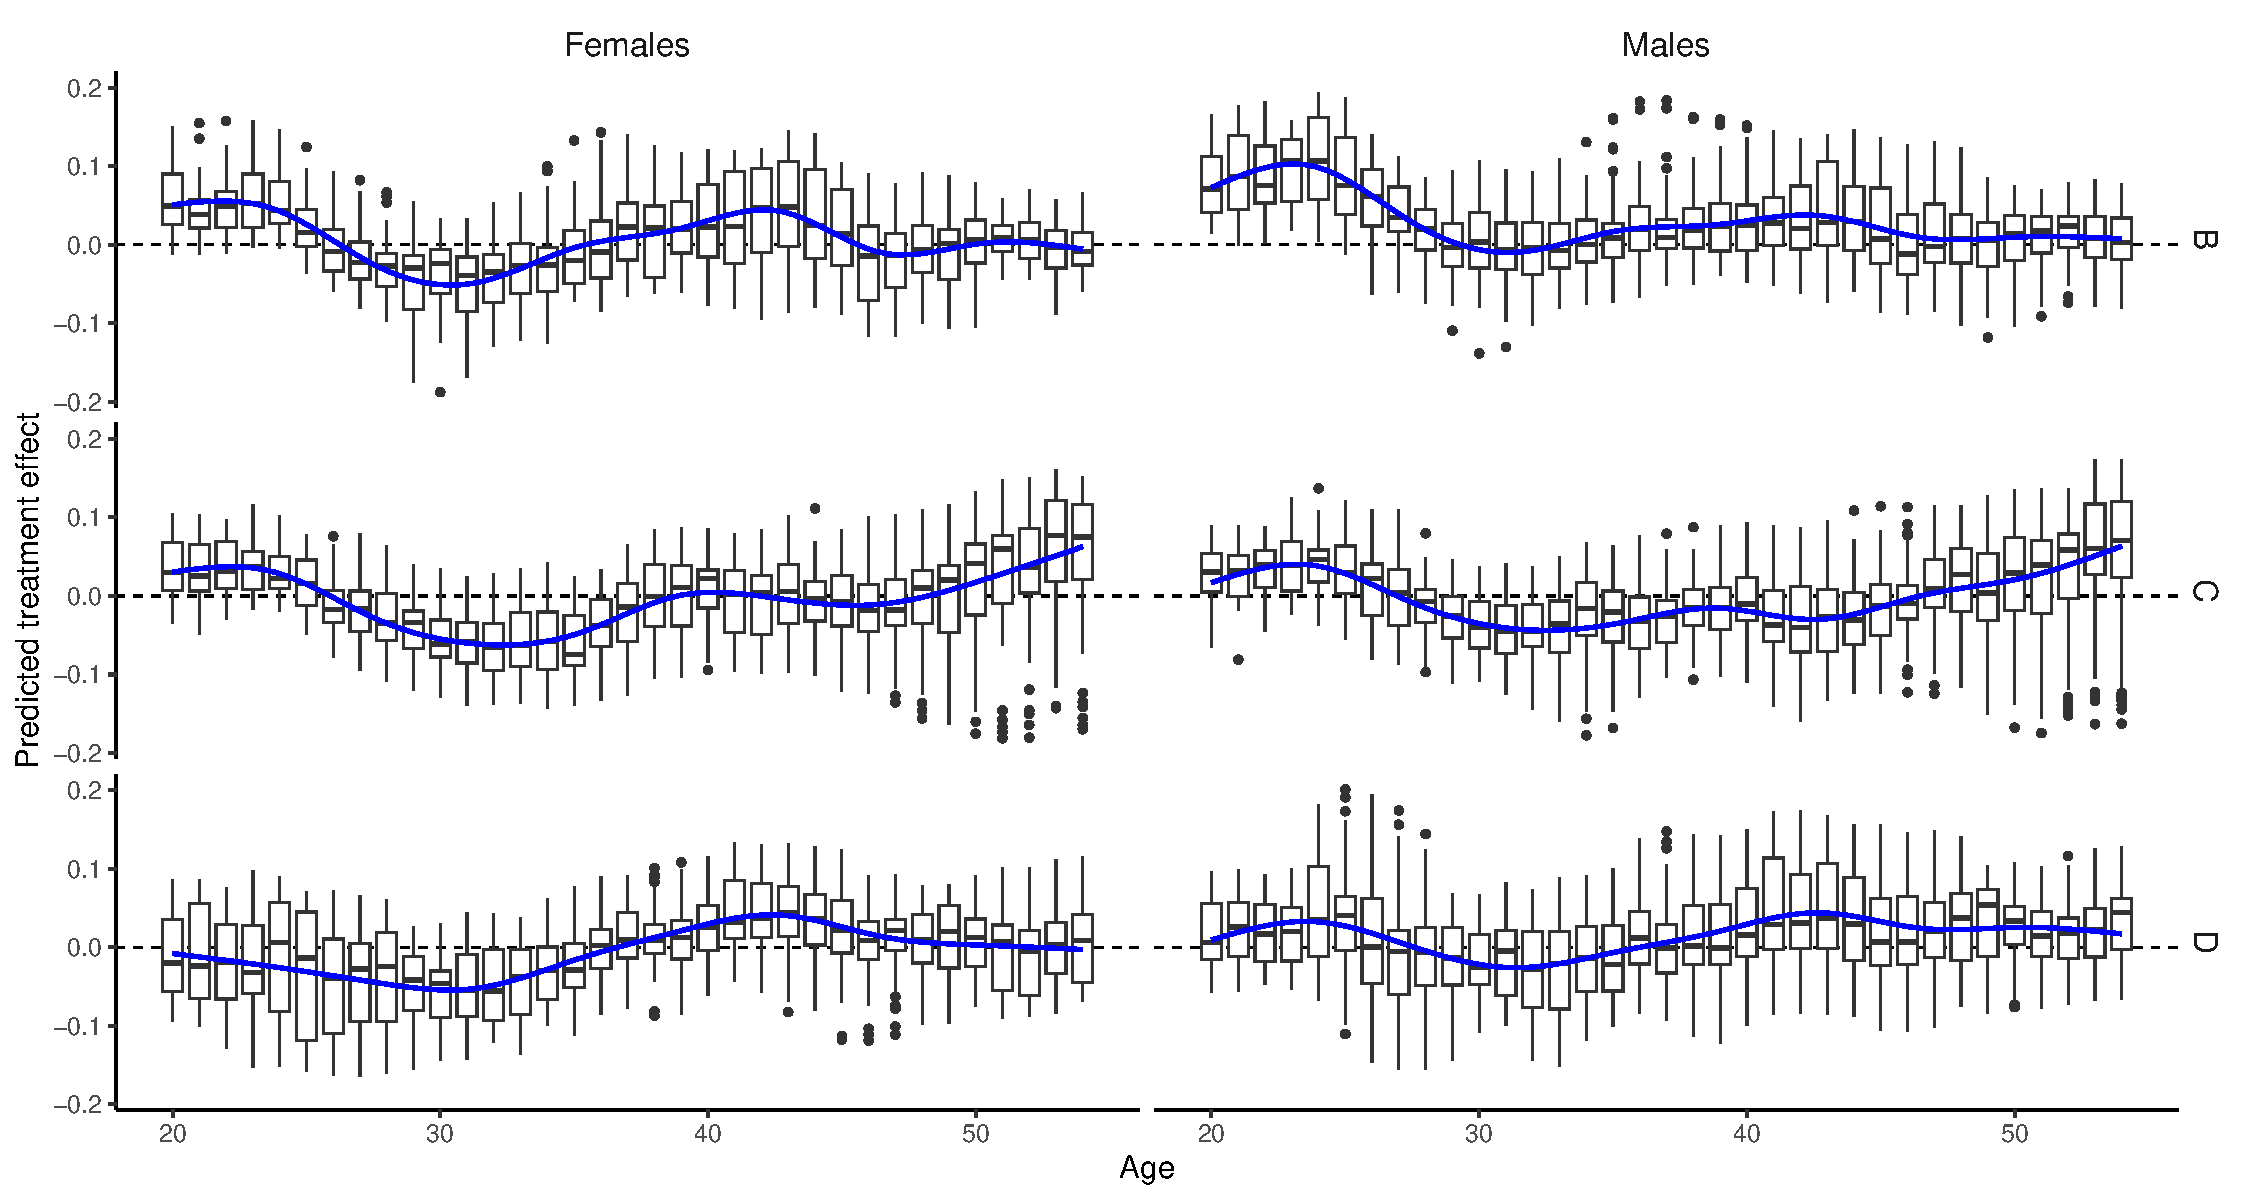
\includegraphics{robustness-body_files/figure-latex/boxplot-rcf-int-1} \caption{Boxplot of Predicted Treatment Effects by Gender and Age. Notes: Blue fitted line represents GAM smoothing. Covariates are gender, age, number of past coordinations, number of hospitals per 10 square kilometers, number of hospitals with PBSC collection per 10 square kilometers and number of hospitals with BM collection per 10 square kilometers.}\label{fig:boxplot-rcf-int}
\end{figure}

Figure \ref{fig:boxplot-rcf-int} plots the distribution of predicted treatment effects for each experimental group by age. Notably, the effect of experimental group B is positive for all males under the age of 25. As a result, the RCF shows that the average effect of experimental group B for men in their 20s is \(12.1\) points, which is close to the results of the subsample analysis of the linear probability model presented in Figure \ref{fig:coefplot-reg-stock-subset} (see Table \ref{tab:rcf-int-cate}).

For other genders and ages, the message effects are heterogeneous. For example, for some men in their 30s and 40s, the effect of experimental group B is more than 10 percentage points. They live in areas with a relatively large number of hospitals and have lower travelling costs for coordination and donation (see Table \ref{tab:rcf-middle-male}). Experimental group C, with only the Early Coordination message added, has a negative effect for most women in their early 30s. For men and women in their late 40s and older, the median effect of Experimental Group C is positive, but widely distributed.\footnote{Surprisingly, among men and women in this age group, those for whom experimental group C has a positive effect live in areas with relatively fewer hospitals (higher travelling costs) (see Tables \ref{tab:rcf-older-male} and \ref{tab:rcf-older-female}).}

\begin{table}

\caption{\label{tab:rcf-int-corr}Correlation of Predicted Treatment Effects}
\centering
\fontsize{9}{11}\selectfont
\begin{threeparttable}
\begin{tabular}[t]{lcccccccc}
\toprule
\multicolumn{1}{c}{ } & \multicolumn{8}{c}{Treatment effect of D} \\
\cmidrule(l{3pt}r{3pt}){2-9}
\multicolumn{1}{c}{ } & \multicolumn{2}{c}{Female} & \multicolumn{2}{c}{Male} & \multicolumn{2}{c}{Female} & \multicolumn{2}{c}{Male} \\
\cmidrule(l{3pt}r{3pt}){2-3} \cmidrule(l{3pt}r{3pt}){4-5} \cmidrule(l{3pt}r{3pt}){6-7} \cmidrule(l{3pt}r{3pt}){8-9}
\multicolumn{1}{c}{ } & \multicolumn{1}{c}{Age < 30} & \multicolumn{1}{c}{30 < Age} & \multicolumn{1}{c}{Age < 30} & \multicolumn{1}{c}{30 < Age} & \multicolumn{1}{c}{Age < 30} & \multicolumn{1}{c}{30 < Age} & \multicolumn{1}{c}{Age < 30} & \multicolumn{1}{c}{30 < Age} \\
\cmidrule(l{3pt}r{3pt}){2-2} \cmidrule(l{3pt}r{3pt}){3-3} \cmidrule(l{3pt}r{3pt}){4-4} \cmidrule(l{3pt}r{3pt}){5-5} \cmidrule(l{3pt}r{3pt}){6-6} \cmidrule(l{3pt}r{3pt}){7-7} \cmidrule(l{3pt}r{3pt}){8-8} \cmidrule(l{3pt}r{3pt}){9-9}
  & (1) & (2) & (3) & (4) & (5) & (6) & (7) & (8)\\
\midrule
(Intercept) & \num{-0.038}*** & \num{0.007}*** & \num{-0.016}*** & \num{0.014}*** & \num{-0.035}*** & \num{0.006}*** & \num{0.004}* & \num{0.010}***\\
 & (\num{0.002}) & (\num{0.001}) & (\num{0.002}) & (\num{0.001}) & (\num{0.002}) & (\num{0.001}) & (\num{0.002}) & (\num{0.001})\\
(B + C) & \num{0.339}*** & \num{0.368}*** & \num{0.369}*** & \num{0.430}*** &  &  &  & \\
 & (\num{0.020}) & (\num{0.008}) & (\num{0.018}) & (\num{0.007}) &  &  &  \vphantom{1} & \\
B &  &  &  &  & \num{0.017} & \num{0.409}*** & \num{-0.063}** & \num{0.619}***\\
 &  &  &  &  & (\num{0.035}) & (\num{0.014}) & (\num{0.029}) & (\num{0.015})\\
C &  &  &  &  & \num{0.724}*** & \num{0.329}*** & \num{0.923}*** & \num{0.299}***\\
 &  &  &  &  & (\num{0.036}) & (\num{0.013}) & (\num{0.032}) & (\num{0.011})\\
\addlinespace[0.3em]
\multicolumn{9}{l}{\textit{Linear combination test (F-test)}}\\
\hspace{1em}(B + C) - 1 & \num{-0.661}*** & \num{-0.632}*** & \num{-0.631}*** & \num{-0.570}*** &  &  &  & \\
\hspace{1em} & (\num{0.020}) & (\num{0.008}) & (\num{0.018}) & (\num{0.007}) &  &  &  & \\
\hspace{1em}B - C &  &  &  &  & \num{-0.707}*** & \num{0.079}*** & \num{-0.985}*** & \num{0.319}***\\
\hspace{1em} &  &  &  &  & (\num{0.061}) & (\num{0.022}) & (\num{0.050}) & (\num{0.022})\\
\midrule
Num.Obs. & \num{1132} & \num{3018} & \num{1566} & \num{5333} & \num{1132} & \num{3018} & \num{1566} & \num{5333}\\
\bottomrule
\end{tabular}
\begin{tablenotes}
\item Notes: * p < 0.1, ** p < 0.05, *** p < 0.01. The robust standard errors are in parentheses. 
\end{tablenotes}
\end{threeparttable}
\end{table}

In addition to examining heterogeneity, we discuss the mechanism of experimental arm D using the treatment effects predicted by the RCF. To test the effects of cognitive load due to information overload, experimental arm D adds both the Probability message (experimental arm B) and the Early Coordination message (experimental arm C).

If the matched donor fully understands the information in experimental arm D, the effect of experimental group D should be the sum of the effects of experimental arms B and C. To test this point, columns (1)--(4) of Table \ref{tab:rcf-int-corr} regress the predicted treatment effect of experimental arm D on the sum of the predicted effects of experimental arms B and C. For each gender and age group, a 1-point increase in the sum of the effects of experimental arms B and C increases the effect of experimental group D by 0.3--0.4 points. Since we can reject the null hypothesis that the coefficient on the sum of the predicted effects of experimental arms B and C is 1 (that the sum of their predicted effects is equal to the effect of experimental arm D), this suggests that the matched donors do not fully understand the information in experimental arm D and are cognitively overloaded due to information overload.

A matched donor who does not completely receive information would either value either the Probability message or the Early Coordination message, or would discount the two pieces of information equally. To test this point, columns (4)--(8) of Table \ref{tab:rcf-int-corr} regress the predicted treatment effects of experimental arm D on the predicted effects of experimental arm B and of experimental arm C. The results show that for men and women in their 20s, the partial correlations between experimental arms C and D are stronger than those between experimental arms B and D, which is statistically significant different by F-test. This implies that they value the Early Coordination message more than the Probability message. Thus, experimental arm D is ineffective for men in their 20s.

Interestingly, for men and women over 30, the partial correlations between experimental arms C and D are weaker than those between experimental arms B and D, which is statistically significant difference by F-test. In other words, they value the Probability message more than the Early Coordination message. Thus, while the median effect of experimental group C for men and women in their late 40s and older is about 8 points, the median treatment effect of experimental group D is almost zero.

\hypertarget{reply-speed}{%
\subsection{Response Speed to Notification}\label{reply-speed}}

\begin{figure}[t]
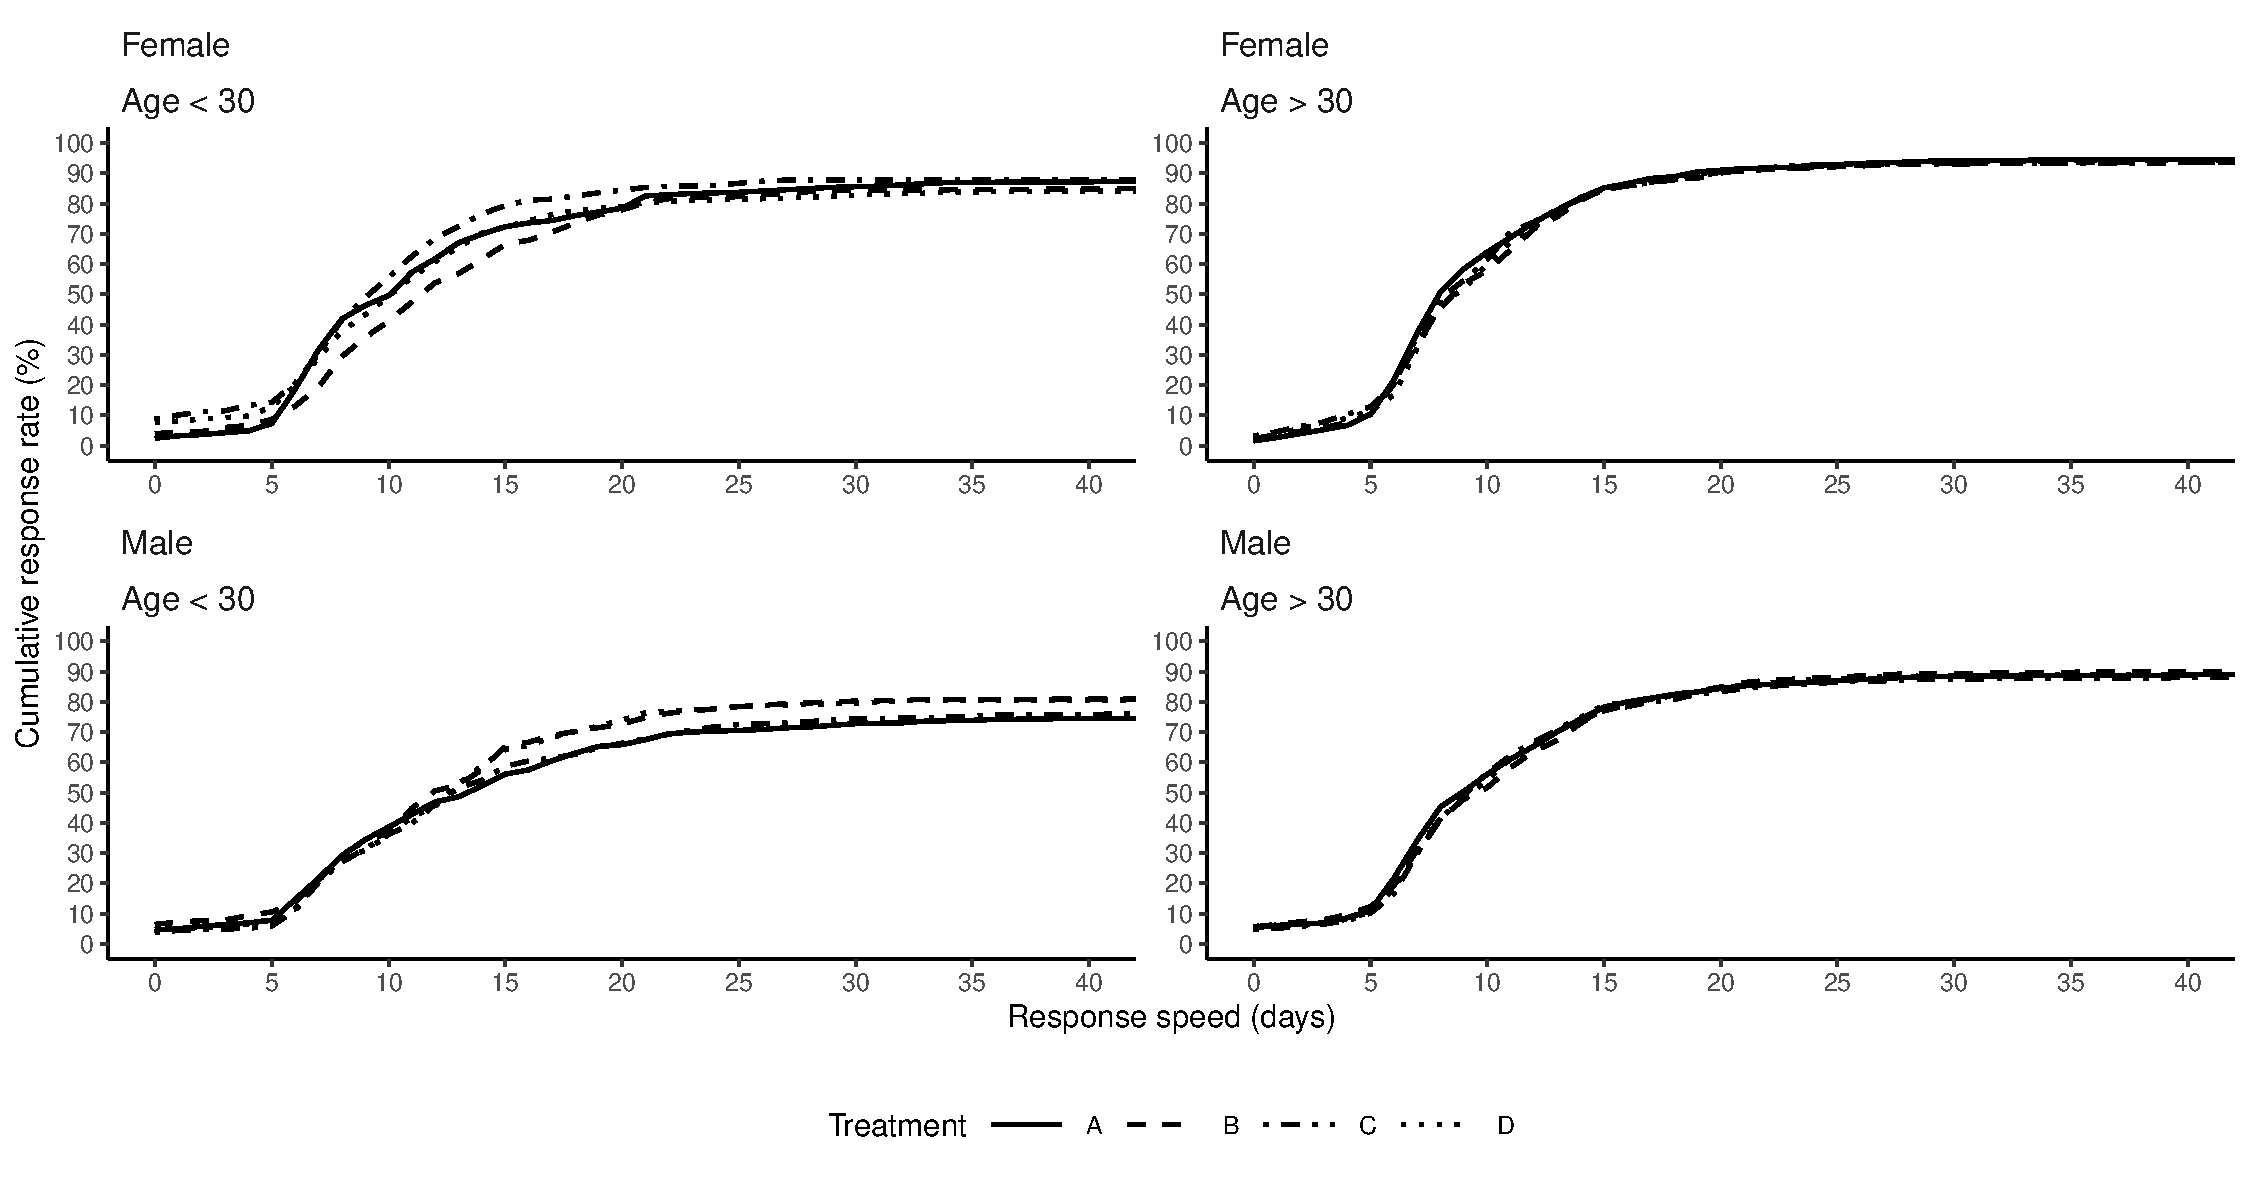
\includegraphics{robustness-body_files/figure-latex/cumulative-response-rate-1} \caption{Cumulative Response Rates by Gender and Age Group.}\label{fig:cumulative-response-rate}
\end{figure}

The Early Coordination message provides the fact that early coordination increases a patient's transplant rate. Therefore, this message may encourage early responses to the compatibility notice. Figure \ref{fig:cumulative-response-rate} shows the cumulative response rate for each day of the 40 days after the match notification was sent. Since the effect on responses is heterogeneous by gender and age, as shown in the previous results, we also split the subsample by gender and age here and focus on the heterogeneity of the effect on quick responses.

\begin{figure}[t]
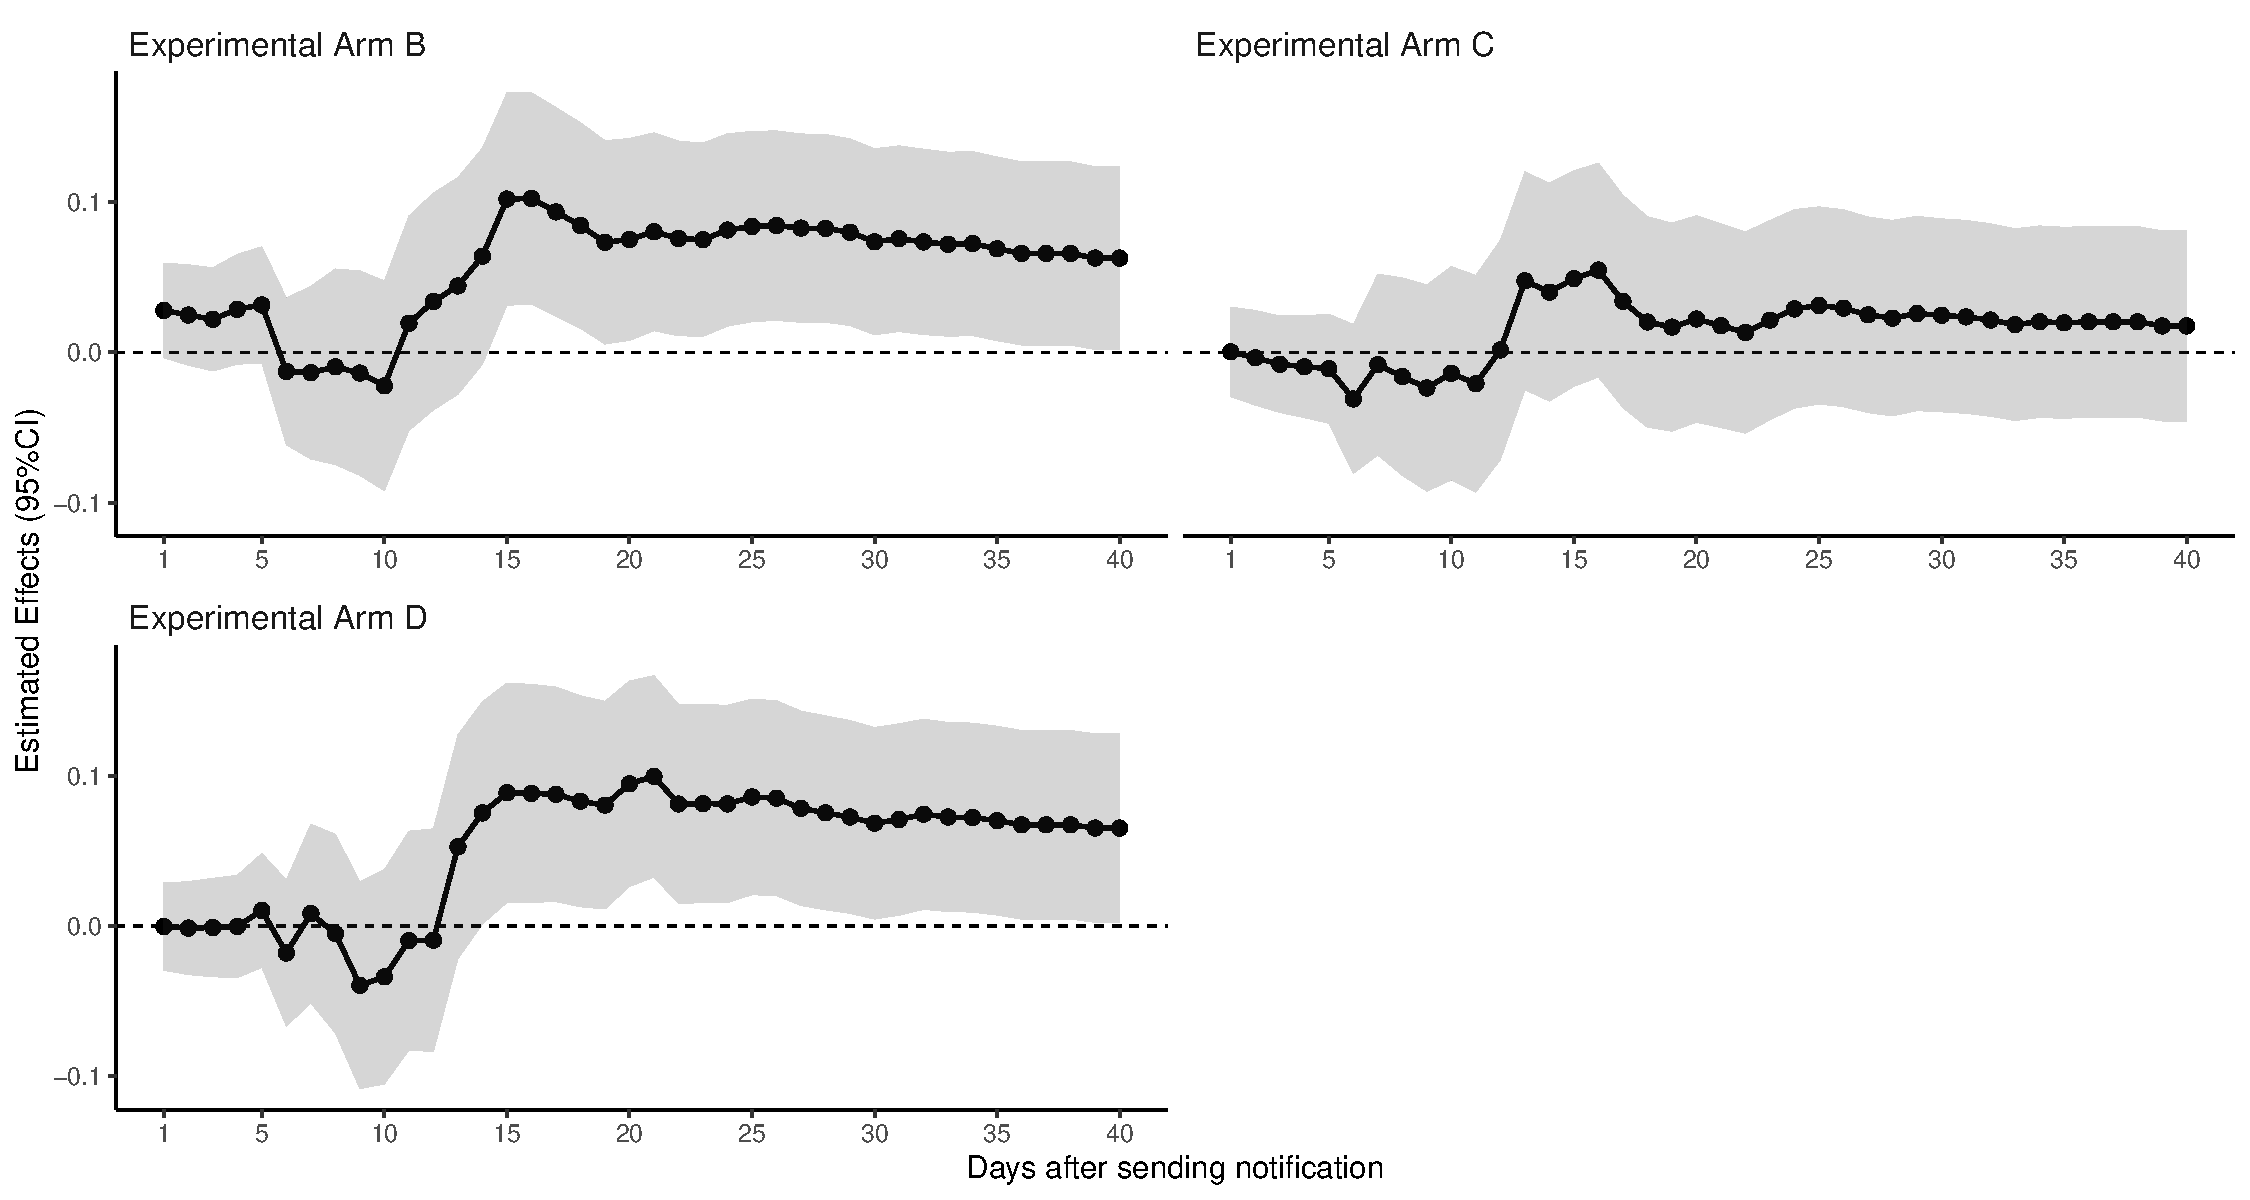
\includegraphics{robustness-body_files/figure-latex/young-male-flow-1} \caption{Effect on Reply within Specific Days after Sending Notification among Males Less than 30. Notes: These plots show the average effect (and associated 95 percent confidential interval) on cumulative responses at sepcific days. We use robust standard errors. We control number of past coordinations, number of hospitals per 10 square kilometers, number of hospitals with PBSC collection per 10 square kilometers, number of hospitals with BM collection per 10 square kilometers, month dummies, and week dummies.}\label{fig:young-male-flow}
\end{figure}

While there are no significant differences in the pattern of cumulative response rates for men and women over 30, there are some notable results for men and women under 30.\footnote{For men and women over 30 years of age, the cumulative response rate for each day differs little between the experimental arms, except for certain periods, and is not statistically significant. See Figure \ref{fig:old-male-flow} and \ref{fig:old-female-flow} in Appendix.} In the group of men in their 20s, 15 days after the compatibility notice was sent, the responses of experimental arms B and D begin to increase relative to the controls. As a result, the cumulative response rate of the two experimental groups is statistically significantly higher than that of the control (Figure \ref{fig:young-male-flow}).\footnote{In the regression analysis, we created a dummy variable that takes 1 if the potential donor responded within \(d\) days as the outcome variable. If the potential donor responded after \(d\) days or did not respond, the outcome variable is 0.} Since the compatibility notice recommends a response within 7 days, a response after 15 days from the mailing of the compatibility notice cannot be considered an early response. Thus, although experimental arms B and D increase the ultimate response rate among men in their 20s, they have no effect on encouraging early responses. This result is natural because the Probability message, the intervention in Experimental Groups B and D, is not intended to encourage early responses. In addition, the trend in experimental arm C, where only Early Coordination messages are added, is almost the same as the control, so it cannot be said that Early Coordination messages encourage early responses in this group.

\begin{figure}[t]
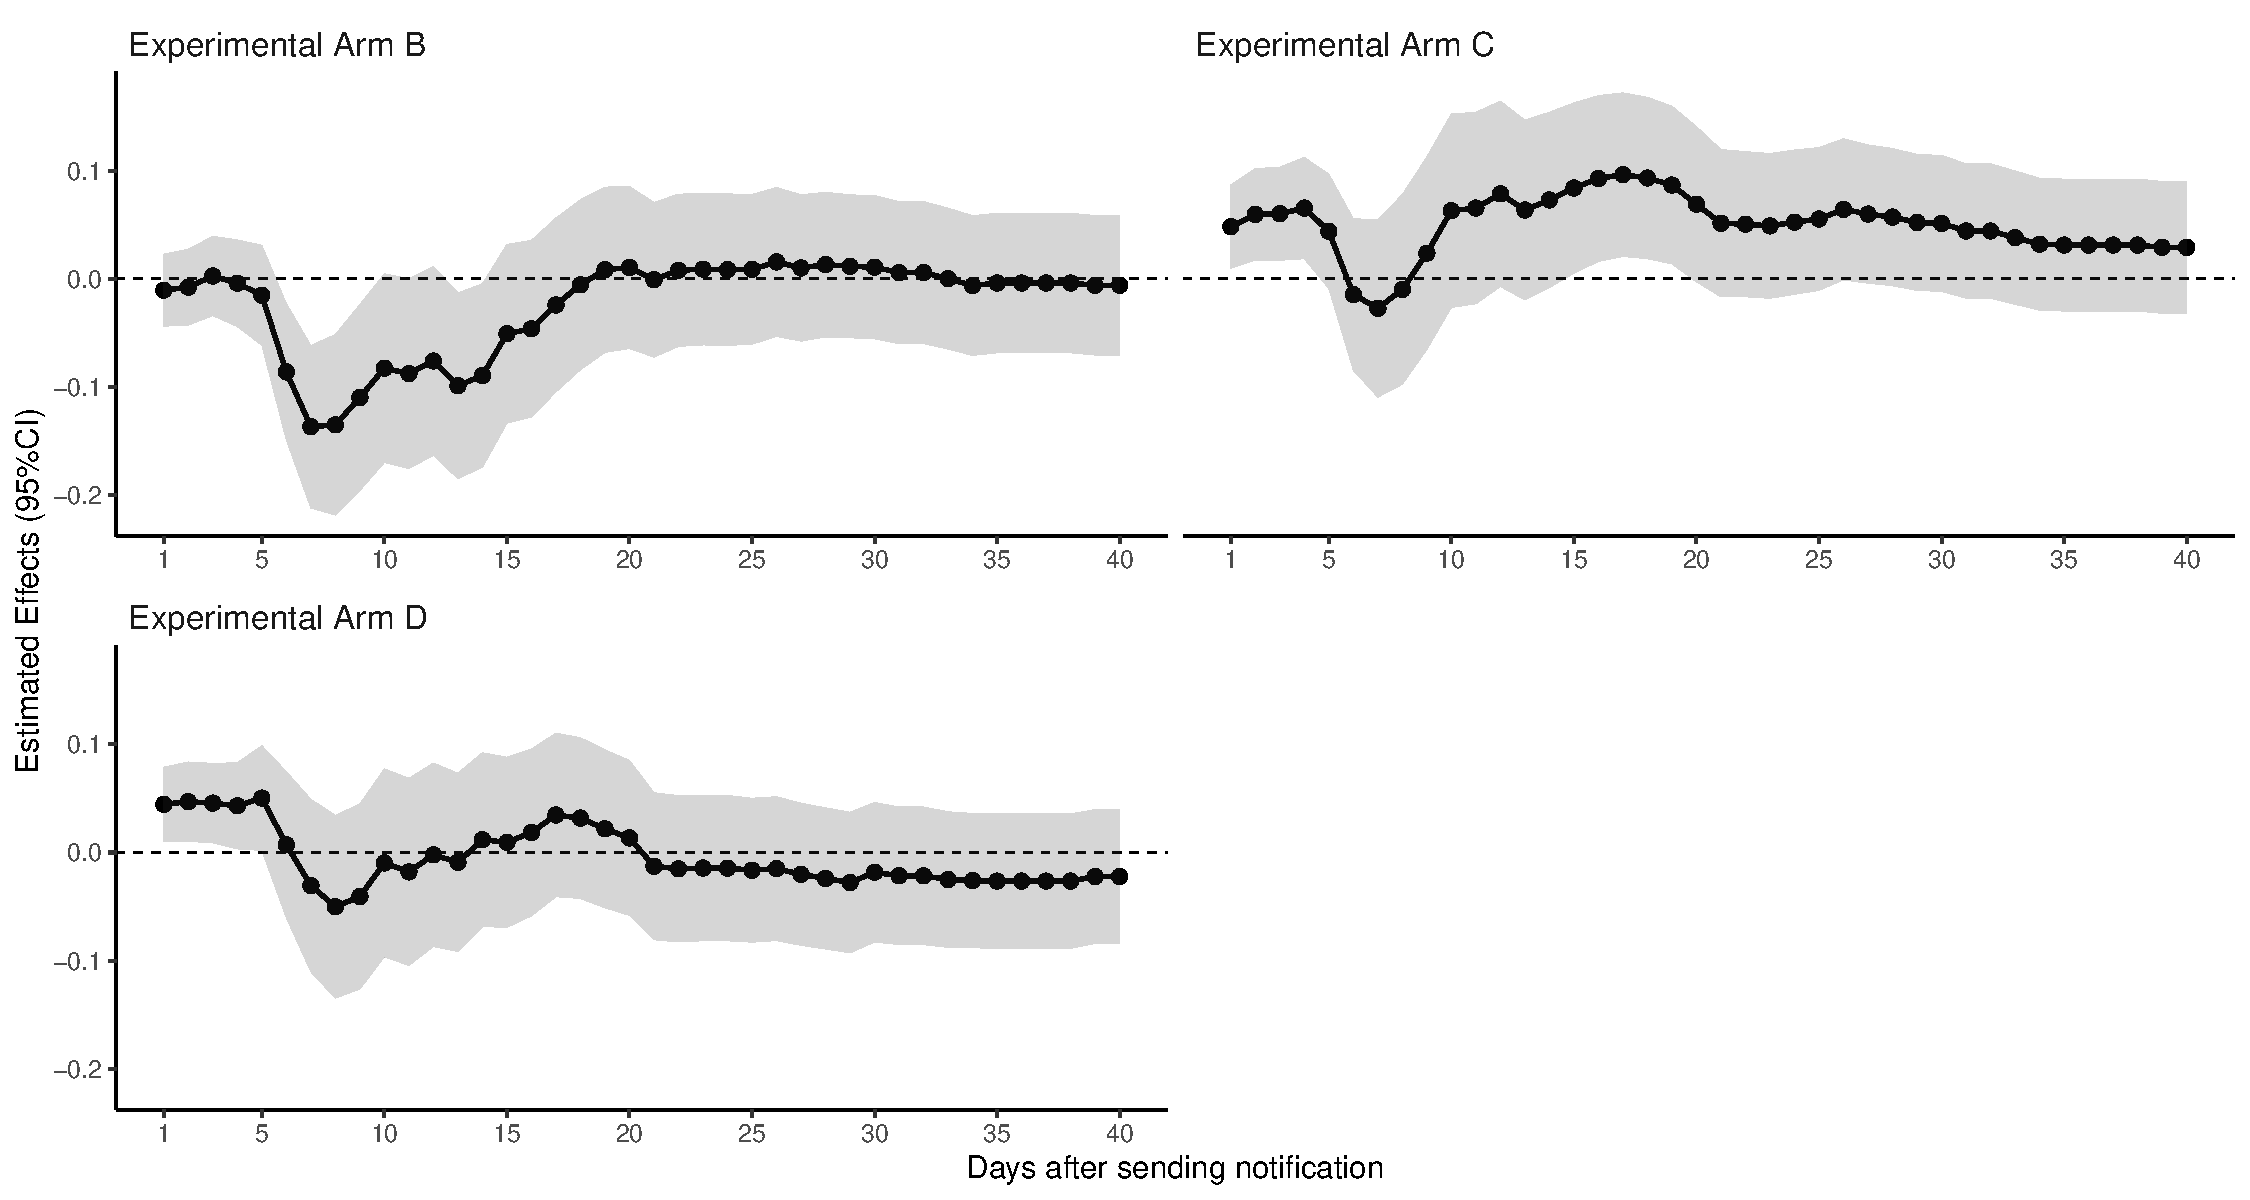
\includegraphics{robustness-body_files/figure-latex/young-female-flow-1} \caption{Effect on Reply within Specific Days after Sending Notification among Females Less than 30. Notes: These plots show the average effect (and associated 95 percent confidential interval) on cumulative responses at sepcific days. We use robust standard errors. We control number of past coordinations, number of hospitals per 10 square kilometers, number of hospitals with PBSC collection per 10 square kilometers, number of hospitals with BM collection per 10 square kilometers, month dummies, and week dummies.}\label{fig:young-female-flow}
\end{figure}

In the 20s female group, the responses of experimental arms C and D, with the addition of the Early Coordination message, increase compared to the control within four days of sending the compatibility message. As a result, the cumulative response rate of the two experimental arms is statistically significantly higher than that of the control (Figure \ref{fig:young-female-flow}). In addition, 10 days after the compatibility notice is sent, the responses of experimental arm C begin to temporarily increase relative to the control, but eventually cease to be statistically significantly different from the cumulative response rate of the control. These results suggest that Early Coordination messages encourage females in their 20s to respond quickly.

\hypertarget{process}{%
\subsection{Effects on the Coordination Process}\label{process}}

Finally, we examine the impact on each step of the coordination process after the response to the compatibility notice. As explained in Section \ref{background}, the coordination process consists of four stages: confirmatory typing, candidate selection, final consent, and collection. We use as outcome variable a dummy variable that takes 1 if a matched donor has reached each stage.

As in the analysis in Section \ref{intention}, we exclude samples in which coordination appears to have been interrupted independently of matched donor willingness. When estimating the effect on confirmatory typing, we exclude cases of interruption for reasons related to the patient. Since the patient's physician is likely to select the healthiest matched donor at the time of candidate selection, cases of interruption for donor health reasons after candidate selection are considered to have occurred independently of the donor's willingness. Thus, when estimating the effects on candidate selection, final consent, and donation, we exclude samples interrupted for patient reasons and samples interrupted for donor health reasons after candidate selection. Note that we should be cautious in our interpretation because sample exclusion alone may not completely eliminate physician decision making. In the control group, 24\% of eligible donors underwent confirmatory testing, 8\% became candidates, and 6\% ultimately donated.

\begin{table}

\caption{\label{tab:est-full-coordination}Linear Probability Model of Coordination}
\centering
\fontsize{9}{11}\selectfont
\begin{threeparttable}
\begin{tabular}[t]{lcccccccc}
\toprule
\multicolumn{1}{c}{ } & \multicolumn{2}{c}{CT} & \multicolumn{2}{c}{Candidate} & \multicolumn{2}{c}{Consent} & \multicolumn{2}{c}{Donation} \\
\cmidrule(l{3pt}r{3pt}){2-3} \cmidrule(l{3pt}r{3pt}){4-5} \cmidrule(l{3pt}r{3pt}){6-7} \cmidrule(l{3pt}r{3pt}){8-9}
  & (1) & (2) & (3) & (4) & (5) & (6) & (7) & (8)\\
\midrule
Treatment B & \num{0.0325}** & \num{0.0326}*** & \num{0.0051} & \num{0.0033} & \num{0.0059} & \num{0.0037} & \num{0.0040} & \num{0.0020}\\
 & (\num{0.0141}) & (\num{0.0073}) & (\num{0.0076}) & (\num{0.0050}) & (\num{0.0074}) & (\num{0.0041}) & (\num{0.0060}) & (\num{0.0043})\\
Treatment C & \num{0.0146} & \num{0.0136} & \num{0.0010} & \num{-0.0023} & \num{0.0024} & \num{-0.0011} & \num{0.0016} & \num{-0.0017}\\
 & (\num{0.0163}) & (\num{0.0087}) & (\num{0.0102}) & (\num{0.0057}) & (\num{0.0086}) & (\num{0.0044}) & (\num{0.0076}) & (\num{0.0047})\\
Treatment D & \num{0.0260} & \num{0.0299}*** & \num{0.0084} & \num{0.0087}* & \num{0.0099} & \num{0.0098}** & \num{0.0030} & \num{0.0029}\\
 & (\num{0.0161}) & (\num{0.0077}) & (\num{0.0093}) & (\num{0.0046}) & (\num{0.0102}) & (\num{0.0048}) & (\num{0.0095}) & (\num{0.0053})\\
\midrule
Control average & 0.2350 & 0.2350 & 0.0779 & 0.0779 & 0.0687 & 0.0687 & 0.0574 & 0.0574\\
Covariates &  & X &  & X &  & X &  & X\\
Num.Obs. & \num{10435} & \num{10435} & \num{8587} & \num{8587} & \num{8558} & \num{8558} & \num{8441} & \num{8441}\\
\bottomrule
\end{tabular}
\begin{tablenotes}
\item Notes: * p < 0.1, ** p < 0.05, *** p < 0.01. The robust standard errors are in parentheses. Covariates are gender, squared polynomial of age, number of past coordinations, number of hospitals per 10 square kilometers, number of hospitals with PBSC collection per 10 square kilometers, number of hospitals with BM collection per 10 square kilometers, month dummies, and week dummies.
\end{tablenotes}
\end{threeparttable}
\end{table}

Table \ref{tab:est-full-coordination} shows the full sample estimation results. The results show that experimental groups B and D, which include probability messages, increase the rate of confirmatory typing by about 3 percentage points, which is a statistically significant effect. This effect is larger than the effect on responses. This is because the likelihood of coordination being interrupted for donor reasons, including health reasons, is lower in experimental groups B and D than in the control group. Thus, although experimental groups B and D do not increase the overall number of people willing to donate, they do maintain the intention to donate, which contributes to the reduction in coordination dropouts.

The effect of experimental groups B and D on the stage after candidate selection is less than 1 percentage point and not statistically significant. This should be interpreted with caution. Since our intervention did not affect demand (number of patients), if our intervention increased the number of people who reached confirmatory typing, it should have increased the number of people who were not selected as candidates for exogenous reasons.

In experimental group B and control group, the number of potential donors who reached confirmatory typing was 774 and 564, respectively. Therefore, experimental group B would have increased the number of confirmatory typings by 210. The number of potential donors who were not selected as candidates due to patient or donor health reasons was 556 in the experimental group B and 385 in the control group. This means that experimental group B has 171 more people who were not selected as candidates for exogenous reasons. Thus, the estimates include not only the effect of our intervention, but also the effect of the demand for stem cell transplants.

\begin{figure}[t]
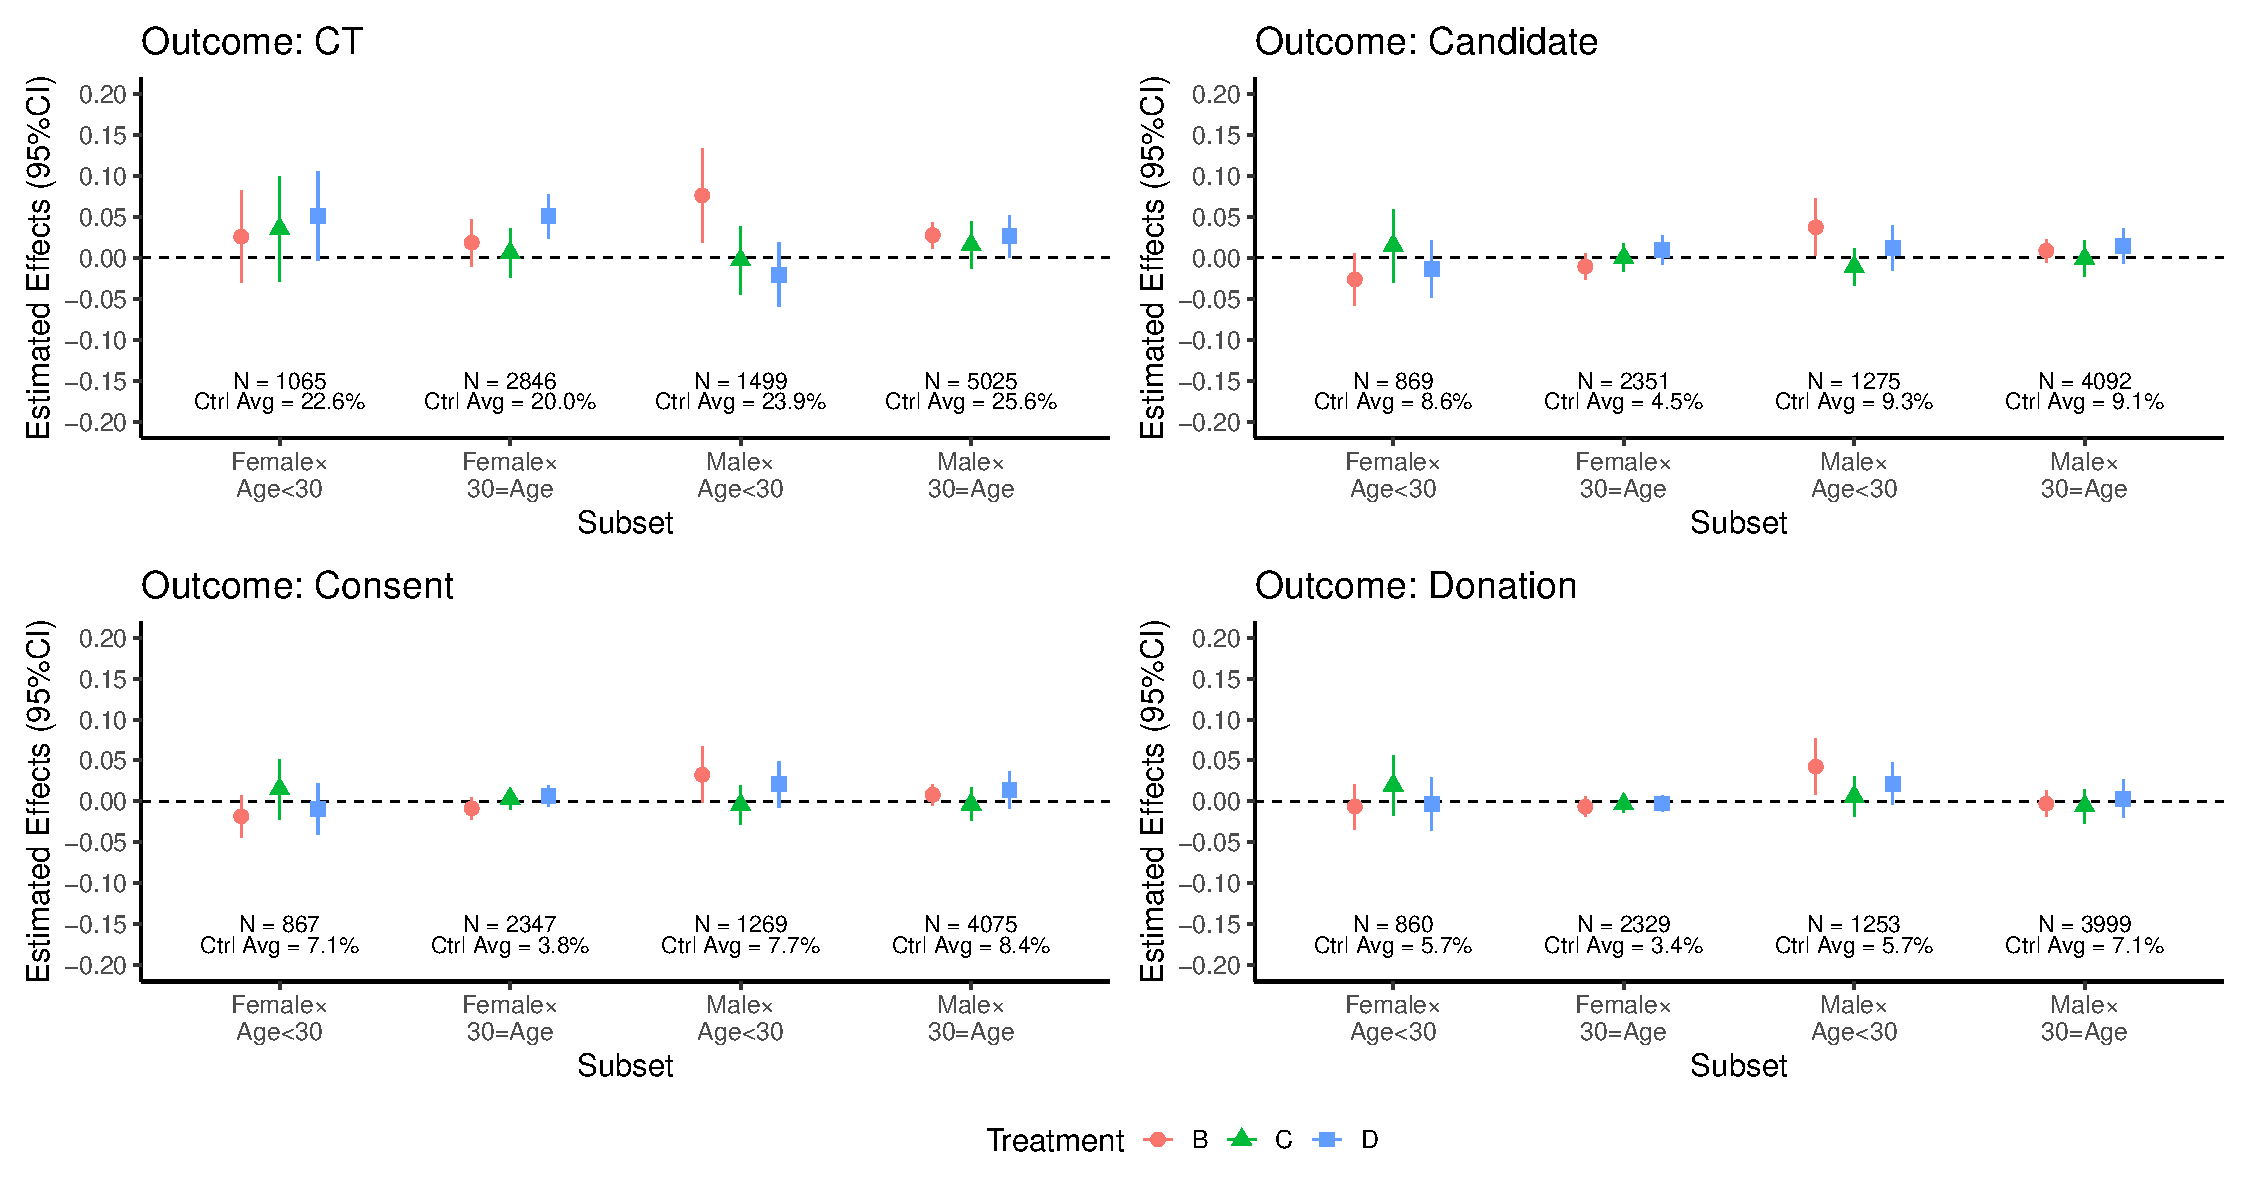
\includegraphics{robustness-body_files/figure-latex/coefplot-reg-subsample-coordination-1} \caption{Effect on Coordination by Gender and Age Group. Note: These plots show the average effect (and associated 95 percent confidential interval) on each outcome by gender and age group. We use robust standard errors. We control number of past coordinations, number of hospitals per 10 square kilometers, number of hospitals with PBSC collection per 10 square kilometers, number of hospitals with BM collection per 10 square kilometers, month dummies, and week dummies.}\label{fig:coefplot-reg-subsample-coordination}
\end{figure}

Figure \ref{fig:coefplot-reg-subsample-coordination} divides the sample into four subsets by gender and age group (under 30 or not) and estimates the message effect in each subset. The results show that experimental group B increases the proportion of men in their 20s who reach confirmatory typing by about 8 percentage points, which is statistically significant. Thus, it is possible that experimental group B not only increases the willingness of men in their 20s to donate, but also maintains it.

Experimental group B has no statistically significant effect on candidate selection and final agreement among men in their 20s. However, the effect on donation is about 4 percentage points and is statistically significant at the 10\% level. As noted earlier, this effect may reflect not only the effect of our intervention, but also the demand for stem cell transplants. If younger males have better transplant outcomes, then the demand for stem cell transplants may be higher in this generation than in other genders and ages. The effect on donation may include this effect. In addition, experimental arm C, which encourages early responses from women in their 20s, has a statistically significant effect on the coordination of this generation.

\hypertarget{conclusion}{%
\section{Discussion and Conclusions}\label{conclusion}}

This study examined the effect of providing information to increase willingness to donate among potential donors enrolled in the JMDP. The results showed that information about the low number of HLA-matched donors per patient (Probability message) increased the willingness to donate among men in their 20s by about 10 percentage points and also increased the rate of achieving confirmatory typing by about 8 percentage points. In addition, this information may increase the transplant rate by 5 percentage points. In terms of numbers, the Probability message increased the number of transplanted donors from 71 to 121.

However, when we simultaneously provide the information that early coordination increases a patient's transplant rate (Early Coordination message), the positive effect of the Probability message disappears because they give more weight to the Early Coordination message in their decision making.

These results suggest that men in their 20s overestimate the number of HLA-matched donors and engage in free-riding behavior. There are two possible reasons for the statistically insignificant effect of the Probability message for the other genders and ages. First, compared to men in their 20s, others may correctly estimate the number of HLA-matched donors. In this case, the Probability message should have no effect on the decision of potential donors.

The second possibility is that the altruistic preferences of men in their 20s differ from those of other genders and age groups. Economic studies suggest that there are two main types of motives for altruistic behavior: warm glow, in which one gain utility from one's own altruistic behavior, and pure altruism, in which one gain utility from the results of altruistic behavior, such as the production of public goods \citep{Andreoni1990}. Those with relatively stronger warm glow are less likely to engage in free-riding behavior because they are less concerned about the actions of others. Thus, compared to men in their 20s, others may have the warm glow preference as the main driver of altruistic behavior. In short, the heterogeneity in the Probability message could be explained by differences in beliefs or motivations.

The Early Coordination message had no effect on the overall response rate among women in their 20s, but had a positive effect on shorter responses (4 days or less). This suggests that it shortens the timing of replies rather than encouraging the response behavior itself. Due to our data limitations, we cannot test whether this message shortens the time to transplant for patients, but it is possible that this information at least contributes to a shorter coordination period.

The lack of effect for other genders and ages may be due to the possibility that others already have this information. Alternatively, women in their 20s may have a stronger degree of present bias and a greater tendency toward delayed behavior than other generations. The heterogeneity of this message effect could be explained by differences in information possession or time preference.

While this study is able to clearly identify the causal effects of information provision through field experiments, it is limited by the fact that the data and experimental design do not allow for the identification of the mechanisms described above, which may be an issue for future work. Nevertheless, this study has practical implications. As discussed in section \ref{intro}, maintaining the intention of potential donors is a challenge for bone marrow donor programs due to the time lag between intention and behavior. In particular, young donors with good transplant outcomes are likely to fail to maintain their intentions and drop out of the program. This study suggests that information provided by the bone marrow donor program office at the time of matching with a patient may promote behavioral change in young potential donors and may be one of the measures to address this problem. In particular, information about the HLA matching of others would increase the efficiency of coordination in the sense that donors with a good transplant performance would be more likely to proceed to coordination. However, some studies \citep[e.g.][]{Switzer2018} have shown that information provision is ineffective, so it is expected that the effectiveness of information provision will be tested in bone marrow donor programs in other countries.

\clearpage

\hypertarget{appendix}{%
\section*{Appendix}\label{appendix}}
\addcontentsline{toc}{section}{Appendix}

\clearpage

\begin{table}

\caption{\label{tab:logit-stock}Logit Model of Reply and Intention}
\centering
\fontsize{9}{11}\selectfont
\begin{threeparttable}
\begin{tabular}[t]{lcccccc}
\toprule
\multicolumn{3}{c}{ } & \multicolumn{4}{c}{Intention} \\
\cmidrule(l{3pt}r{3pt}){4-7}
\multicolumn{1}{c}{ } & \multicolumn{2}{c}{Reply} & \multicolumn{2}{c}{Positive} & \multicolumn{2}{c}{Negative} \\
\cmidrule(l{3pt}r{3pt}){2-3} \cmidrule(l{3pt}r{3pt}){4-5} \cmidrule(l{3pt}r{3pt}){6-7}
  & (1) & (2) & (3) & (4) & (5) & (6)\\
\midrule
Treatment B & \num{1.11} & \num{1.15} & \num{1.09} & \num{1.09} & \num{0.95} & \num{0.97}\\
 & {}[\num{0.94}, \num{1.31}] & {}[\num{0.96}, \num{1.37}] & {}[\num{0.98}, \num{1.22}] & {}[\num{0.98}, \num{1.22}] & {}[\num{0.85}, \num{1.06}] & {}[\num{0.86}, \num{1.09}]\\
Treatment C & \num{0.95} & \num{1.02} & \num{0.98} & \num{0.99} & \num{1.00} & \num{1.03}\\
 & {}[\num{0.80}, \num{1.12}] & {}[\num{0.86}, \num{1.22}] & {}[\num{0.88}, \num{1.09}] & {}[\num{0.88}, \num{1.11}] & {}[\num{0.89}, \num{1.12}] & {}[\num{0.91}, \num{1.16}]\\
Treatment D & \num{1.06} & \num{1.06} & \num{1.02} & \num{1.02} & \num{1.01} & \num{1.00}\\
 & {}[\num{0.89}, \num{1.26}] & {}[\num{0.89}, \num{1.27}] & {}[\num{0.91}, \num{1.14}] & {}[\num{0.91}, \num{1.15}] & {}[\num{0.90}, \num{1.13}] & {}[\num{0.89}, \num{1.13}]\\
\midrule
Covariates &  & X &  & X &  & X\\
Num.Obs. & \num{10985} & \num{10985} & \num{10985} & \num{10985} & \num{10985} & \num{10985}\\
Log.Lik. & \num{-3884.517} & \num{-3712.289} & \num{-7534.803} & \num{-7364.638} & \num{-6945.023} & \num{-6869.968}\\
\bottomrule
\end{tabular}
\begin{tablenotes}
\item Notes: We show odds ratios and associated 95 percent confidential intervals in square brackets. Covariates are gender, squared polynomial of (demeaned) age, number of past coordinations, number of hospitals per 10 square kilometers, number of hospitals with PBSC collection per 10 square kilometers, number of hospitals with BM collection per 10 square kilometers, month dummies, and week dummies.
\end{tablenotes}
\end{threeparttable}
\end{table}

\begin{table}

\caption{\label{tab:logit-coordination}Logit Model of Coordination}
\centering
\fontsize{9}{11}\selectfont
\begin{threeparttable}
\begin{tabular}[t]{lcccccccc}
\toprule
\multicolumn{1}{c}{ } & \multicolumn{2}{c}{CT} & \multicolumn{2}{c}{Candidate} & \multicolumn{2}{c}{Consent} & \multicolumn{2}{c}{Donation} \\
\cmidrule(l{3pt}r{3pt}){2-3} \cmidrule(l{3pt}r{3pt}){4-5} \cmidrule(l{3pt}r{3pt}){6-7} \cmidrule(l{3pt}r{3pt}){8-9}
  & (1) & (2) & (3) & (4) & (5) & (6) & (7) & (8)\\
\midrule
Treatment B & \num{1.19} & \num{1.20} & \num{1.07} & \num{1.04} & \num{1.09} & \num{1.06} & \num{1.07} & \num{1.04}\\
 & {}[\num{1.05}, \num{1.35}] & {}[\num{1.05}, \num{1.36}] & {}[\num{0.86}, \num{1.33}] & {}[\num{0.83}, \num{1.31}] & {}[\num{0.87}, \num{1.38}] & {}[\num{0.83}, \num{1.35}] & {}[\num{0.83}, \num{1.39}] & {}[\num{0.80}, \num{1.35}]\\
Treatment C & \num{1.08} & \num{1.08} & \num{1.01} & \num{0.97} & \num{1.04} & \num{0.99} & \num{1.03} & \num{0.98}\\
 & {}[\num{0.95}, \num{1.23}] & {}[\num{0.94}, \num{1.24}] & {}[\num{0.81}, \num{1.27}] & {}[\num{0.76}, \num{1.23}] & {}[\num{0.82}, \num{1.32}] & {}[\num{0.77}, \num{1.27}] & {}[\num{0.79}, \num{1.34}] & {}[\num{0.74}, \num{1.29}]\\
Treatment D & \num{1.15} & \num{1.18} & \num{1.12} & \num{1.12} & \num{1.16} & \num{1.16} & \num{1.06} & \num{1.05}\\
 & {}[\num{1.01}, \num{1.31}] & {}[\num{1.03}, \num{1.35}] & {}[\num{0.90}, \num{1.40}] & {}[\num{0.89}, \num{1.41}] & {}[\num{0.92}, \num{1.46}] & {}[\num{0.91}, \num{1.47}] & {}[\num{0.81}, \num{1.37}] & {}[\num{0.80}, \num{1.38}]\\
\midrule
Covariates &  & X &  & X &  & X &  & X\\
Num.Obs. & \num{10435} & \num{10435} & \num{8587} & \num{8587} & \num{8558} & \num{8558} & \num{8441} & \num{8441}\\
Log.Lik. & \num{-5909.753} & \num{-5764.480} & \num{-2427.295} & \num{-2349.439} & \num{-2243.901} & \num{-2168.120} & \num{-1906.131} & \num{-1851.371}\\
\bottomrule
\end{tabular}
\begin{tablenotes}
\item Notes: We show odds ratios and associated 95 percent confidential intervals in square brackets. Covariates are gender, squared polynomial of age, number of past coordinations, number of hospitals per 10 square kilometers, number of hospitals with PBSC collection per 10 square kilometers, number of hospitals with BM collection per 10 square kilometers, month dummies, and week dummies.
\end{tablenotes}
\end{threeparttable}
\end{table}

\begin{figure}[t]
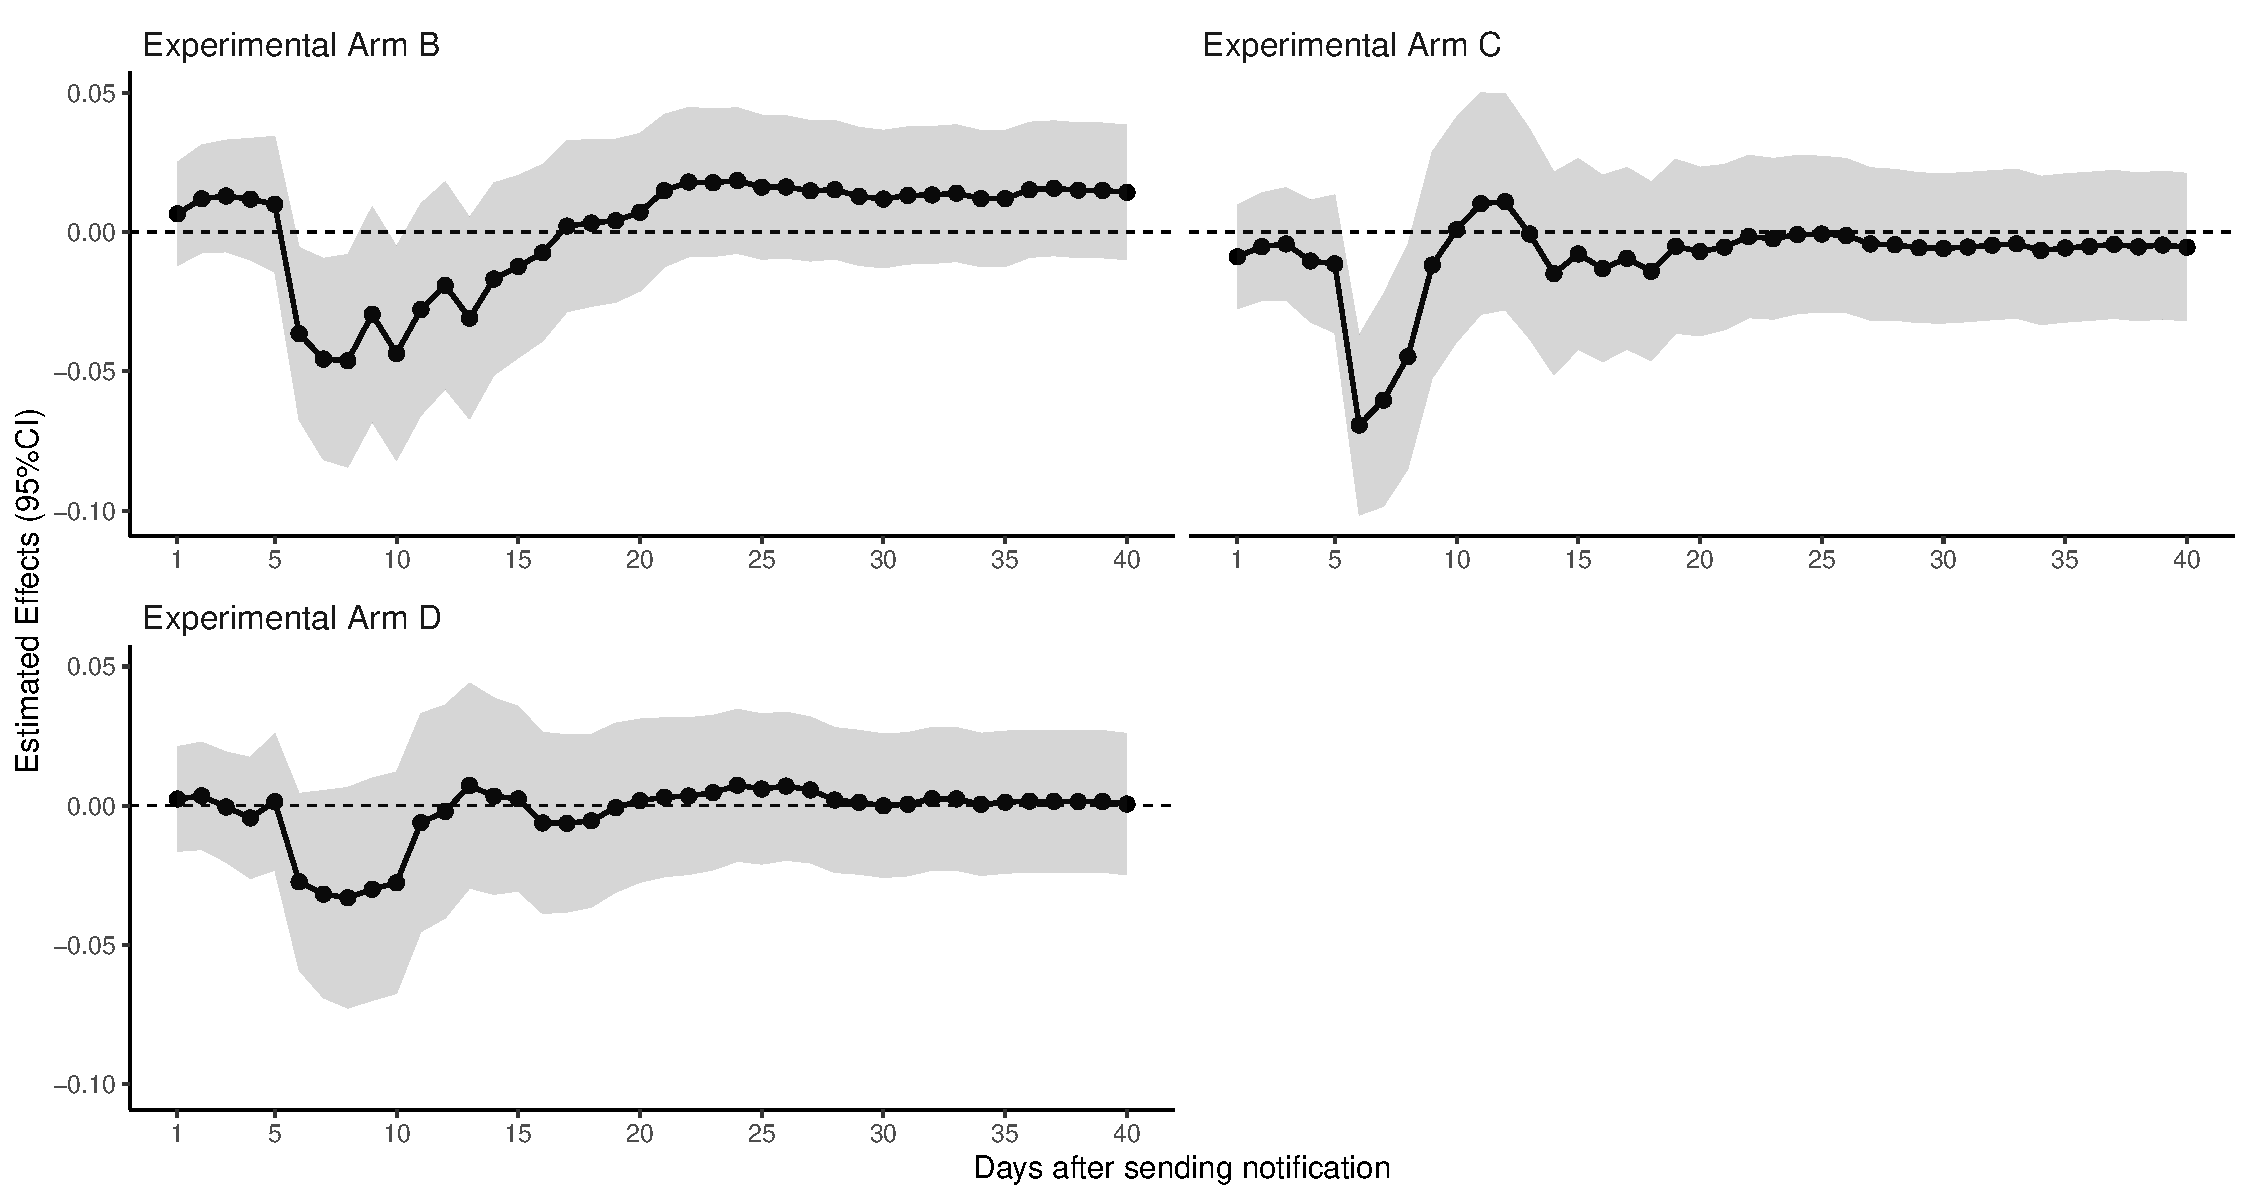
\includegraphics{robustness-body_files/figure-latex/old-male-flow-1} \caption{Effect on Reply within Specific Days after Sending Notification among Males More than 30. Notes: These plots show the average effect (and associated 95 percent confidential interval) on cumulative responses at specific day. We use robust standard errors. We control number of past coordinations, number of hospitals per 10 square kilometers, number of hospitals with PBSC collection per 10 square kilometers, number of hospitals with BM collection per 10 square kilometers, month dummies, and week dummies.}\label{fig:old-male-flow}
\end{figure}

\begin{figure}[t]
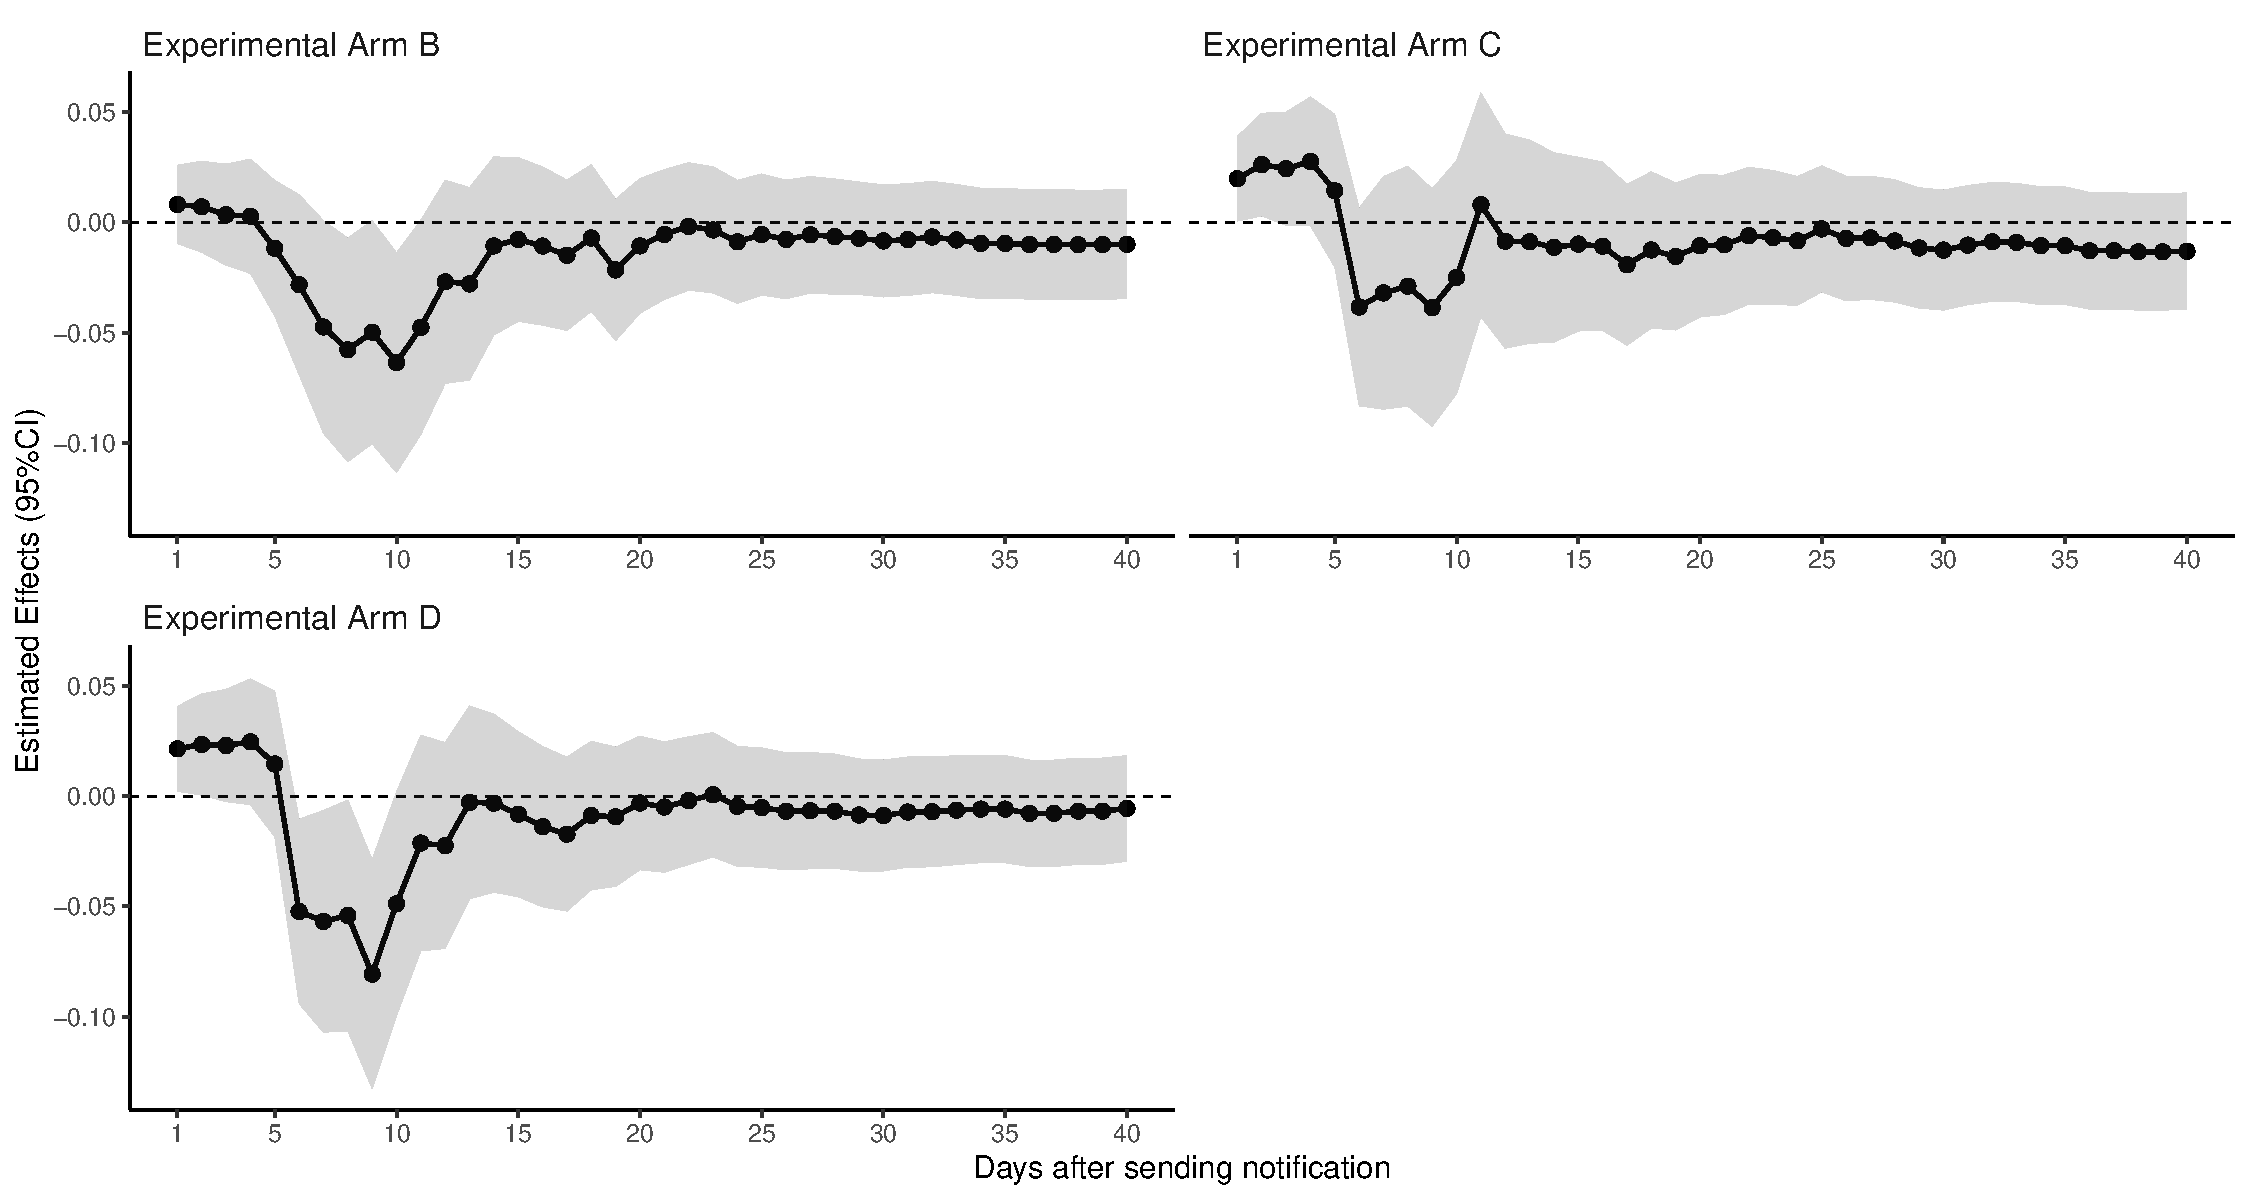
\includegraphics{robustness-body_files/figure-latex/old-female-flow-1} \caption{Effect on Reply within Specific Days after Sending Notification among Females More than 30. Notes: These plots show the average effect (and associated 95 percent confidential interval) on cumulative responses at specific day. We use robust standard errors. We control number of past coordinations, number of hospitals per 10 square kilometers, number of hospitals with PBSC collection per 10 square kilometers, number of hospitals with BM collection per 10 square kilometers, month dummies, and week dummies.}\label{fig:old-female-flow}
\end{figure}

\begin{table}

\caption{\label{tab:rcf-int-cate}Conditional Average Treatment Effect Estimated by RCF}
\centering
\fontsize{9}{11}\selectfont
\begin{threeparttable}
\begin{tabular}[t]{lcccc}
\toprule
\multicolumn{1}{c}{ } & \multicolumn{2}{c}{Female} & \multicolumn{2}{c}{Male} \\
\cmidrule(l{3pt}r{3pt}){2-3} \cmidrule(l{3pt}r{3pt}){4-5}
\multicolumn{1}{c}{ } & \multicolumn{1}{c}{Age < 30} & \multicolumn{1}{c}{30 < Age} & \multicolumn{1}{c}{Age < 30} & \multicolumn{1}{c}{30 < Age} \\
\cmidrule(l{3pt}r{3pt}){2-2} \cmidrule(l{3pt}r{3pt}){3-3} \cmidrule(l{3pt}r{3pt}){4-4} \cmidrule(l{3pt}r{3pt}){5-5}
 & (1) & (2) & (3) & (4)\\
\midrule
B & -0.0045 & -0.0102 & 0.1243*** & 0.0181\\
 & (0.0468) & (0.0287) & (0.0399) & (0.0215)\\
C & 0.0450 & -0.0154 & 0.0475 & -0.0117\\
 & (0.0475) & (0.0298) & (0.0408) & (0.0228)\\
D & -0.0546 & 0.0023 & 0.0490 & 0.0224\\
 & (0.0470) & (0.0291) & (0.0398) & (0.0221)\\
\bottomrule
\end{tabular}
\begin{tablenotes}
\item Notes: * p < 0.1, ** p < 0.05, *** p < 0.01. Standard errors are in parentheses. See Athey and Wager (2019) for estimation method of conditional average treatment effect (CATE). Since these estimates are asymptotically normal, we calculate z-score under the null hypothesis that CATE is zero, and obtain p-value. 
\end{tablenotes}
\end{threeparttable}
\end{table}

\begin{table}

\caption{\label{tab:rcf-middle-male}Sample Characteristics of Predicted Treatment Effect of Arm B (Middle-aged Males)}
\centering
\fontsize{9}{11}\selectfont
\begin{threeparttable}
\begin{tabular}[t]{lccc}
\toprule
\multicolumn{1}{c}{ } & \multicolumn{2}{c}{Predicted treatment effect} & \multicolumn{1}{c}{ } \\
\cmidrule(l{3pt}r{3pt}){2-3}
\multicolumn{1}{c}{ } & \multicolumn{1}{c}{Effect < 0.1} & \multicolumn{1}{c}{0.1 < Effect} & \multicolumn{1}{c}{P-value} \\
\cmidrule(l{3pt}r{3pt}){2-2} \cmidrule(l{3pt}r{3pt}){3-3} \cmidrule(l{3pt}r{3pt}){4-4}
 & (1) & (2) & (3)\\
\midrule
Age & 35.679 & 37.515 & < 0.001\\
Number of past coordinations & 1.652 & 2.660 & < 0.001\\
Number of listed hospitals & 0.396 & 1.407 & < 0.001\\
Number of hospitals listed with PBSC collection & 0.133 & 0.486 & < 0.001\\
Number of hospitals listed with BM collection & 0.199 & 0.836 & < 0.001\\
N & 9101 & 1948 & \\
\bottomrule
\end{tabular}
\begin{tablenotes}
\item Notes: Column (1) and (2) show average sample characteristics. Column (3) shows p-values of difference-in-means test. We use males with 30-39 age.
\end{tablenotes}
\end{threeparttable}
\end{table}

\begin{table}

\caption{\label{tab:rcf-older-male}Sample Characteristics of Predicted Treatment Effect of Arm C (Older Males)}
\centering
\fontsize{9}{11}\selectfont
\begin{threeparttable}
\begin{tabular}[t]{lccc}
\toprule
\multicolumn{1}{c}{ } & \multicolumn{2}{c}{Predicted treatment effect} & \multicolumn{1}{c}{ } \\
\cmidrule(l{3pt}r{3pt}){2-3}
\multicolumn{1}{c}{ } & \multicolumn{1}{c}{Non-positive} & \multicolumn{1}{c}{Positive} & \multicolumn{1}{c}{P-value} \\
\cmidrule(l{3pt}r{3pt}){2-2} \cmidrule(l{3pt}r{3pt}){3-3} \cmidrule(l{3pt}r{3pt}){4-4}
 & (1) & (2) & (3)\\
\midrule
Age & 48.681 & 49.923 & < 0.001\\
Number of past coordinations & 1.801 & 1.861 & 0.303\\
Number of listed hospitals & 0.570 & 0.397 & < 0.001\\
Number of hospitals listed with PBSC collection & 0.193 & 0.134 & < 0.001\\
Number of hospitals listed with BM collection & 0.320 & 0.186 & < 0.001\\
N & 9054 & 1995 & \\
\bottomrule
\end{tabular}
\begin{tablenotes}
\item Notes: Column (1) and (2) show average sample characteristics. Column (3) shows p-values of difference-in-means test. We use males with over 45 age.
\end{tablenotes}
\end{threeparttable}
\end{table}

\begin{table}

\caption{\label{tab:rcf-older-female}Sample Characteristics of Predicted Treatment Effect of Arm C (Older Females)}
\centering
\fontsize{9}{11}\selectfont
\begin{threeparttable}
\begin{tabular}[t]{lccc}
\toprule
\multicolumn{1}{c}{ } & \multicolumn{2}{c}{Predicted treatment effect} & \multicolumn{1}{c}{ } \\
\cmidrule(l{3pt}r{3pt}){2-3}
\multicolumn{1}{c}{ } & \multicolumn{1}{c}{Non-positive} & \multicolumn{1}{c}{Positive} & \multicolumn{1}{c}{P-value} \\
\cmidrule(l{3pt}r{3pt}){2-2} \cmidrule(l{3pt}r{3pt}){3-3} \cmidrule(l{3pt}r{3pt}){4-4}
 & (1) & (2) & (3)\\
\midrule
Age & 48.442 & 50.133 & < 0.001\\
Number of past coordinations & 1.666 & 1.533 & 0.041\\
Number of listed hospitals & 0.528 & 0.440 & 0.029\\
Number of hospitals listed with PBSC collection & 0.157 & 0.164 & 0.633\\
Number of hospitals listed with BM collection & 0.281 & 0.225 & 0.019\\
N & 9993 & 1056 & \\
\bottomrule
\end{tabular}
\begin{tablenotes}
\item Notes: Column (1) and (2) show average sample characteristics. Column (3) shows p-values of difference-in-means test. We use females with over 45 age.
\end{tablenotes}
\end{threeparttable}
\end{table}

\clearpage

\renewcommand\refname{References}
  \bibliography{biblio.bib}

\end{document}
